\section*{Anhang}
\addcontentsline{toc}{section}{Anhang}
\subsection*{Technische Aspekte der Simulation}\label{sec:ap_tec}
\addcontentsline{toc}{subsection}{Technische Aspekte der Simulation}
\subsubsection*{Allgemeiner Aufbau des Projekts}
Diese Arbeit und die dazugehörige Simulation wurden im Zuge des Seminars \emph{Moderne Mathematik: Mathematisches Modellieren} im Sommersemester 2016 erstellt. Beide liegen unter Versionsverwaltung als Git-Repository und sind öffentlich unter \url{http://github.com/themetalone/ss16momaparkingproblem} einsehbar. Zum Zeitpunkt dieser Arbeit steht der Inhalt des Repositorys unter der \emph{MIT Lizenz}.

\subsubsection*{Implementierung der Simulation}
Die Simulation ist in der Programmiersprache \emph{Java 8} geschrieben und lauffähig unter \emph{JRE 1.8}. Es wird die Projektverwaltung \emph{Maven} verwendet, eine Veröffentlichung auf \emph{Maven Central} ist nicht vorgesehen. 

Im Gegensatz zu dem doch sehr einfachen Strukturdiagramm in Abbildung \ref{fig_simOver} ist der tatsächliche Aufbau der Simulation wesentlich komplexer und verfolgt die Prinzipien von maximaler Bindung und minimaler Kopplung. Um eine geringe Kopplung, also eine geringe Abhängigkeit der Simulationskomponenten untereinander, zu gewährleisten, werden Klassenhierarchien und Verteilerklassen verwendet. Erst durch die Verwendung einer Konfigurationsdatei, einer sogenannten \emph{Spring Beans} Konfiguration, wird eine Verbindung zwischen den verschiedenen Objekten einer Simulation hergestellt. Dadurch wird es möglich mehrere Simulationen mit verschiedenem Aufbau und Parametern zu starten, ohne am Quellcode der Simulation Änderungen vornehmen zu müssen. Ebenso werden Erweiterungen des Simulation um zusätzliche Heuristiken oder andere Straßentopologien vereinfacht. 

Um auch mehrere große Simulationen zeitsparender abarbeiten zu können werden Multi-Kern Prozessoren unterstützt. 

Während der Simulation werden die folgenden Daten erhoben:
\begin{itemize}
	\item Bei der Erzeugung
	\begin{itemize}
		\item Eines Parkplatzes: ID und Entfernung zum Ziel
		\item Eines Fahrzeuges: ID und verwendete Heuristik
	\end{itemize}
	\item Wenn geparkt wird
	\begin{itemize}
		\item den aktuellen Zustand des gesamten Parkplatzes
		\item die ID des parkenden Autos, die Entfernung und die Simulationszeit
		\item die Heuristik, die den Parkplatz ausgewählt hat, ihre Parameter, die Entfernung und die Simulationszeit
	\end{itemize}
\end{itemize}
Für die Datenhaltung wurde eine \emph{H2-SQL} Datenbank gewählt. 

\subsubsection*{How-To}
\begin{description}
	\item[Beschaffen des Frameworks:] Auf der Website \url{https://github.com/themetalone/SS16MoMaParkingProblem/releases} die Datei \texttt{parking.simulation-0.0.1-SNAPSHOT-runnable.jar} laden. Möchte man die Simulation um neue Klassen erweitern und verwendet \emph{Maven}, genügt die Datei \texttt{parking.simulation-0.0.1-SNAPSHOT-framework.jar}
	\item[Beschaffen des Quellcodes:] \url{https://github.com/themetalone/SS16MoMaParkingProblem/archive/master.zip}
	\item[Simulation mit Laden einer Konfiguration:] Durch setzen der Systemvariable \texttt{cfg} mit \texttt{-Dcfg=``spring-config.xml''} im Aufruf der Jar Datei, wobei \texttt{spring-config.xml} die Konfigurationsdatei ist.
\end{description}

\subsubsection*{Verwendete Technologien}
\begin{itemize}
	\item SimpleLoggerFacade4Java \url{http://www.slf4j.org/}
	\item The Apache Commons Mathematics Library \url{http://commons.apache.org/proper/commons-math/}
	\item H2 Database Engine \url{http://www.h2database.com/html/main.html}
	\item Spring Framework \url{https://spring.io/}
\end{itemize}
\subsection*{Streudiagramme der Ergebnisse}
\addcontentsline{toc}{subsection}{Streudiagramme der Ergebnisse}
Die Streudiagramme dieser Arbeit wurden mit der Website \href{http:plot.ly/plot}{Plotly} erzeugt.
\subsubsection*{Einzelner lernender Fahrer}
\begin{figure}[H]
	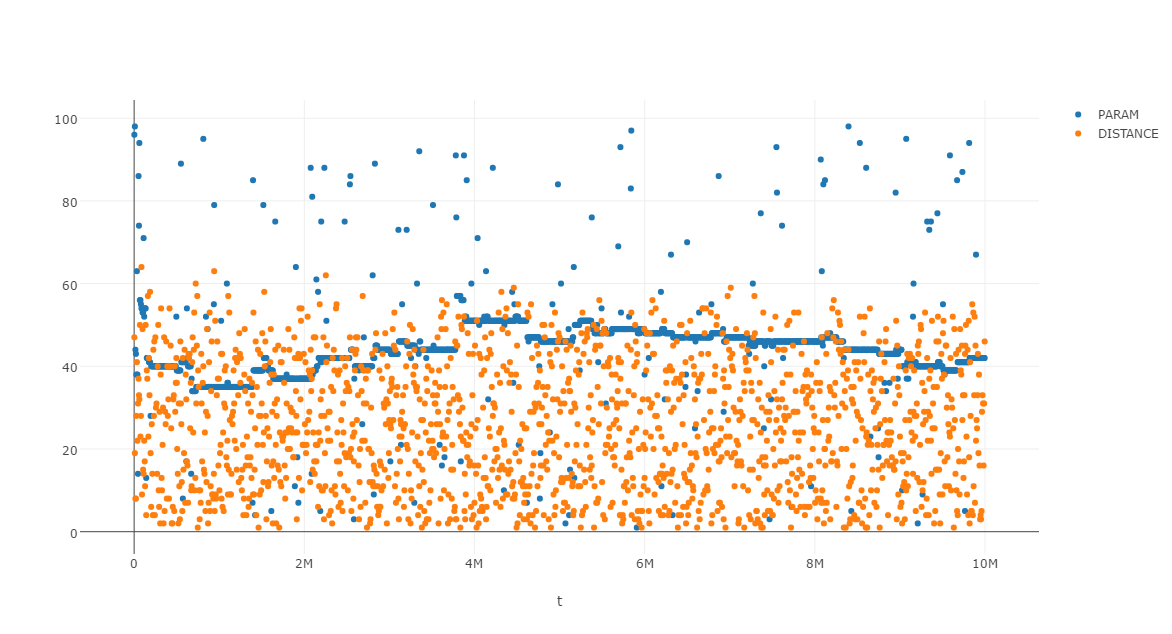
\includegraphics[width=0.8\textwidth]{analyse/SingleMutant/blockcount1.png}
	\caption{\emph{Block-Count}-Heuristik bei 1 Auto pro Minute und einem lernenden Fahrer}\label{fig:ap_sm_bc_1}
\end{figure}
\begin{figure}[H]
	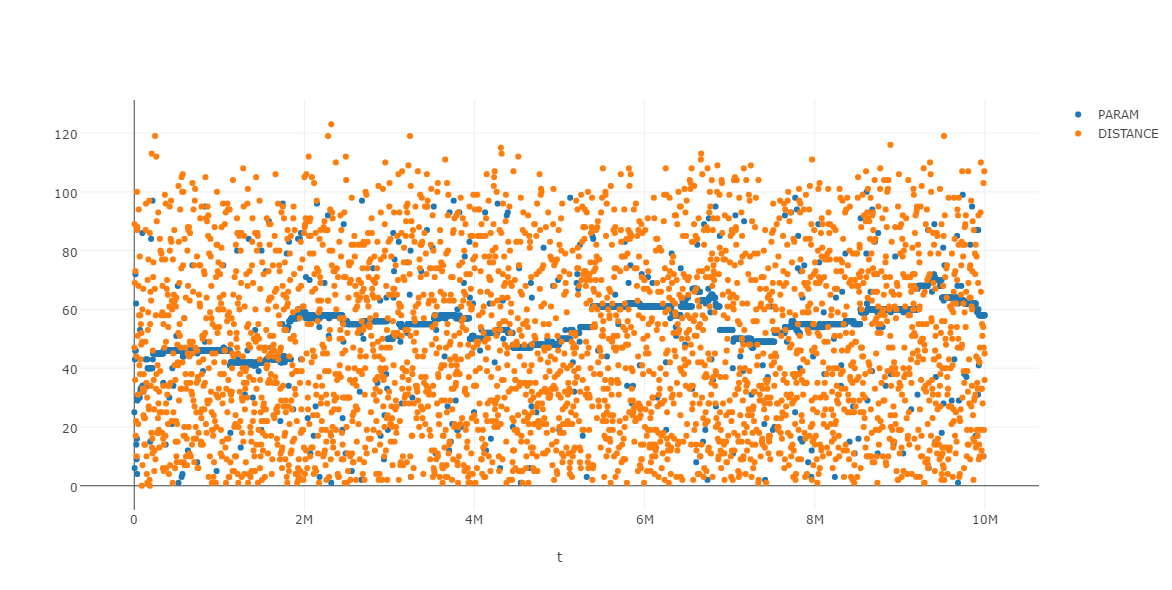
\includegraphics[width=0.8\textwidth]{analyse/SingleMutant/blockcount2.png}
	\caption{\emph{Block-Count}-Heuristik bei 2 Autos pro Minute und einem lernenden Fahrer}\label{fig:ap_sm_bc_2}
\end{figure}
\begin{figure}[H]
	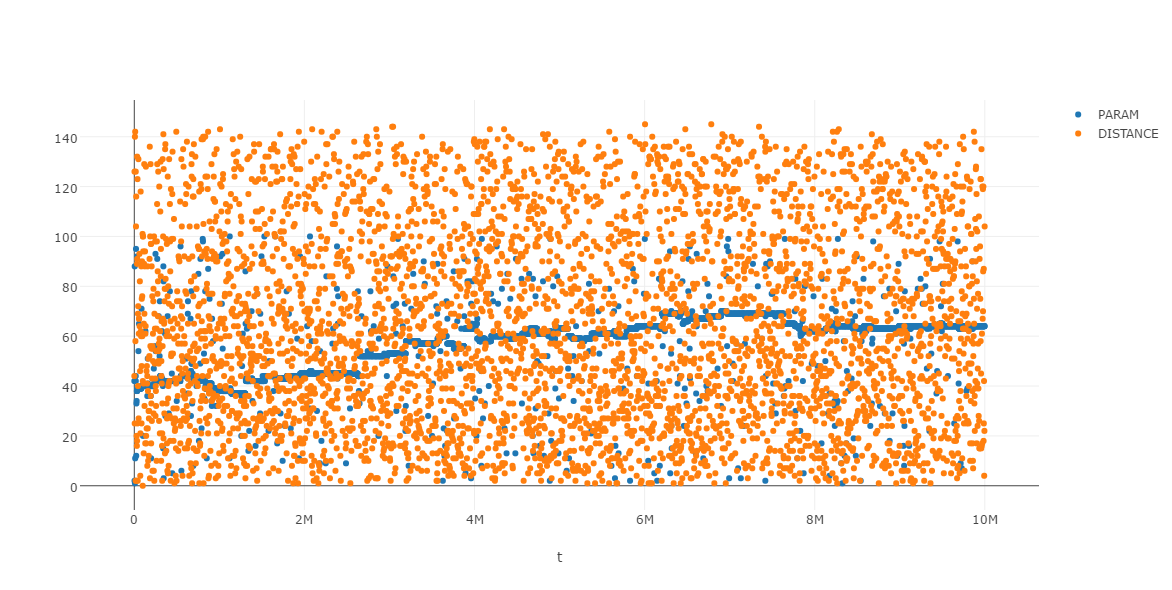
\includegraphics[width=0.8\textwidth]{analyse/SingleMutant/blockcount4.png}
	\caption{\emph{Block-Count}-Heuristik bei 4 Autos pro Minute und einem lernenden Fahrer}\label{fig:ap_sm_bc_4}
\end{figure}
\begin{figure}[H]
	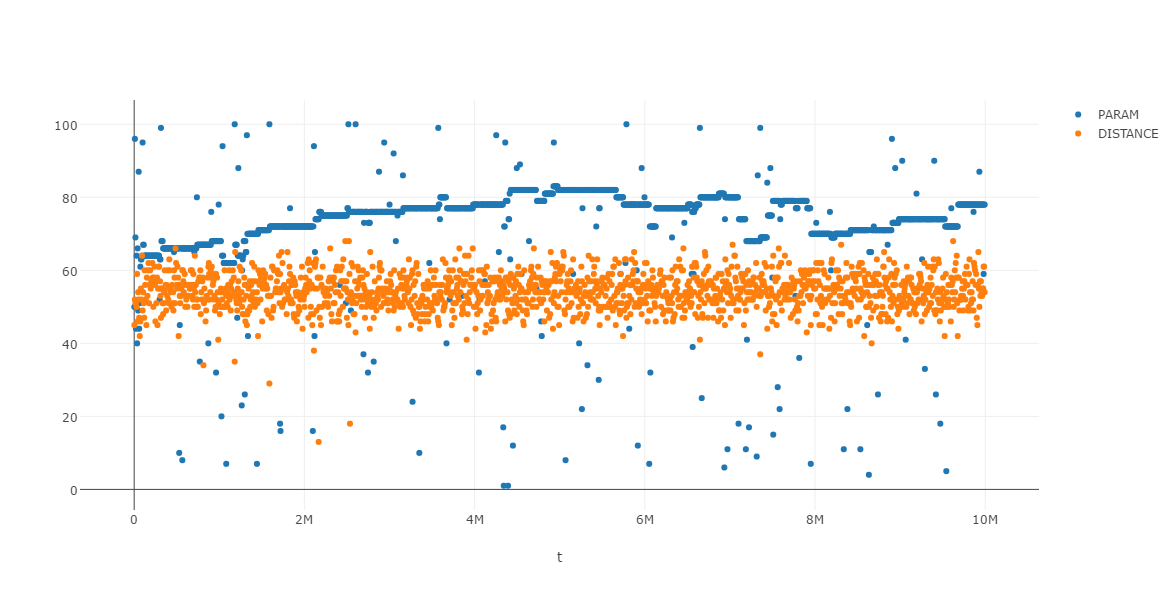
\includegraphics[width=0.8\textwidth]{analyse/SingleMutant/carcount1.png}
	\caption{\emph{Car-Count}-Heuristik bei 1 Auto pro Minute und einem lernenden Fahrer}\label{fig:ap_sm_cc_1}
\end{figure}
\begin{figure}[H]
	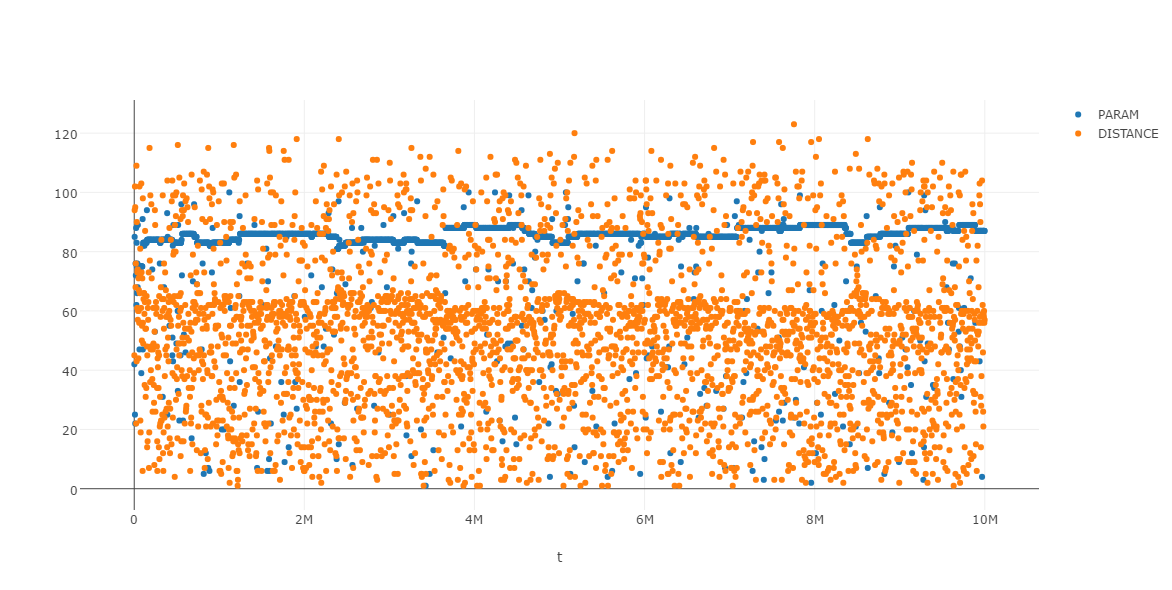
\includegraphics[width=0.8\textwidth]{analyse/SingleMutant/carcount2.png}
	\caption{\emph{Car-Count}-Heuristik bei 2 Autos pro Minute und einem lernenden Fahrer}\label{fig:ap_sm_cc_2}
\end{figure}
\begin{figure}[H]
	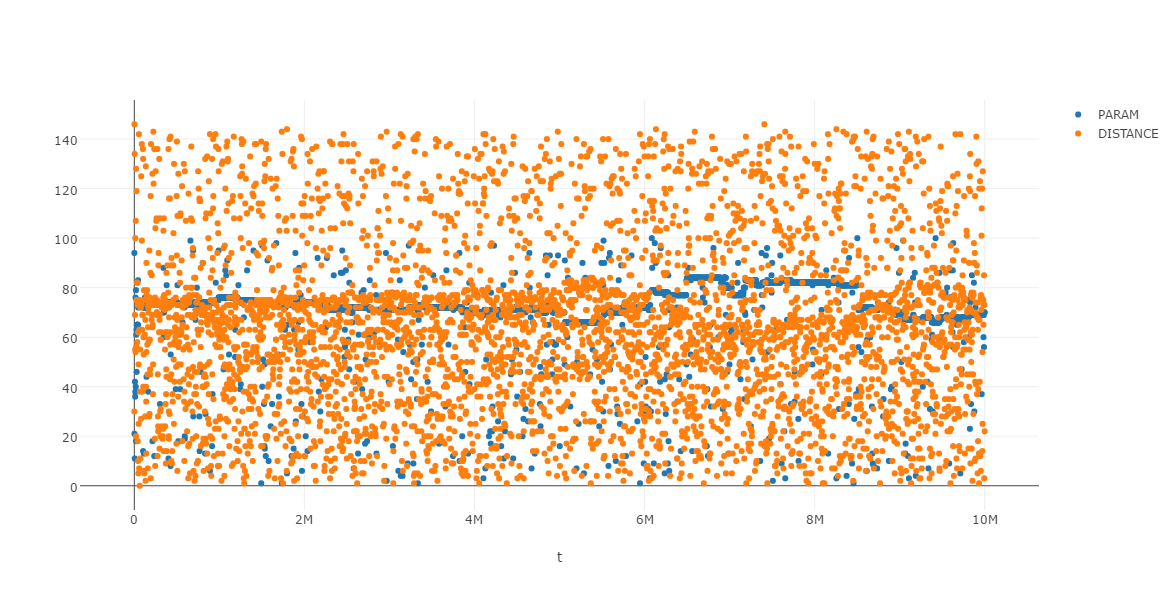
\includegraphics[width=0.8\textwidth]{analyse/SingleMutant/carcount4.png}
	\caption{\emph{Car-Count}-Heuristik bei 4 Autos pro Minute und einem lernenden Fahrer}\label{fig:ap_sm_cc_4}
\end{figure}
\begin{figure}[H]
	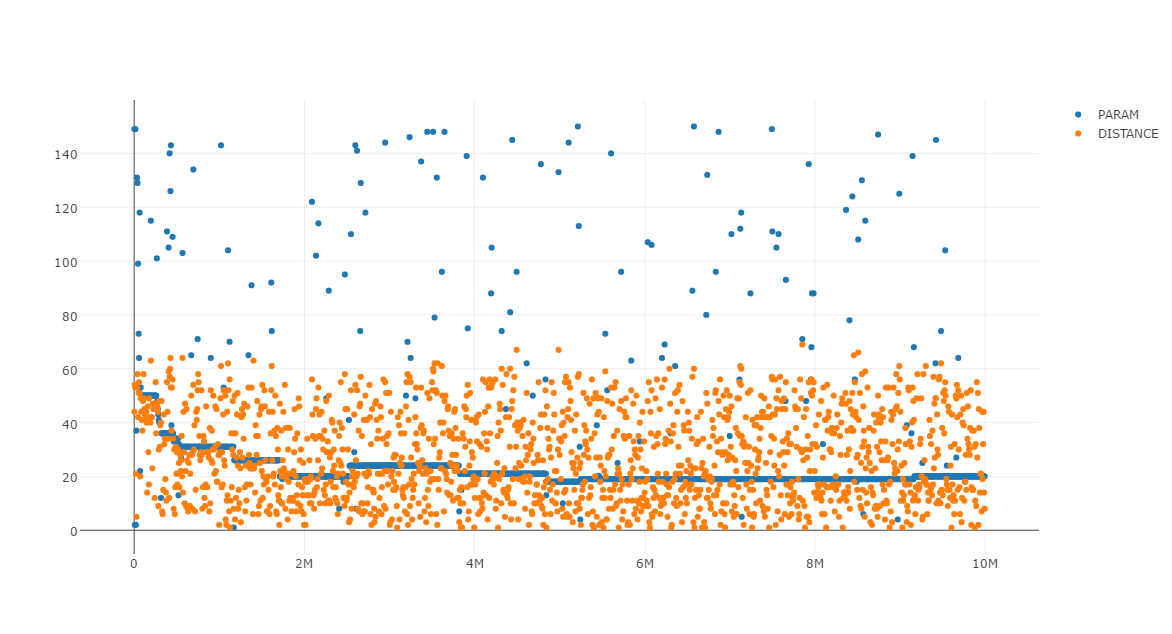
\includegraphics[width=0.8\textwidth]{analyse/SingleMutant/fixeddistance1.png}
	\caption{\emph{Fixed-Distance}-Heuristik bei 1 Auto pro Minute und einem lernenden Fahrer}\label{fig:ap_sm_fd_1}
\end{figure}
\begin{figure}[H]
	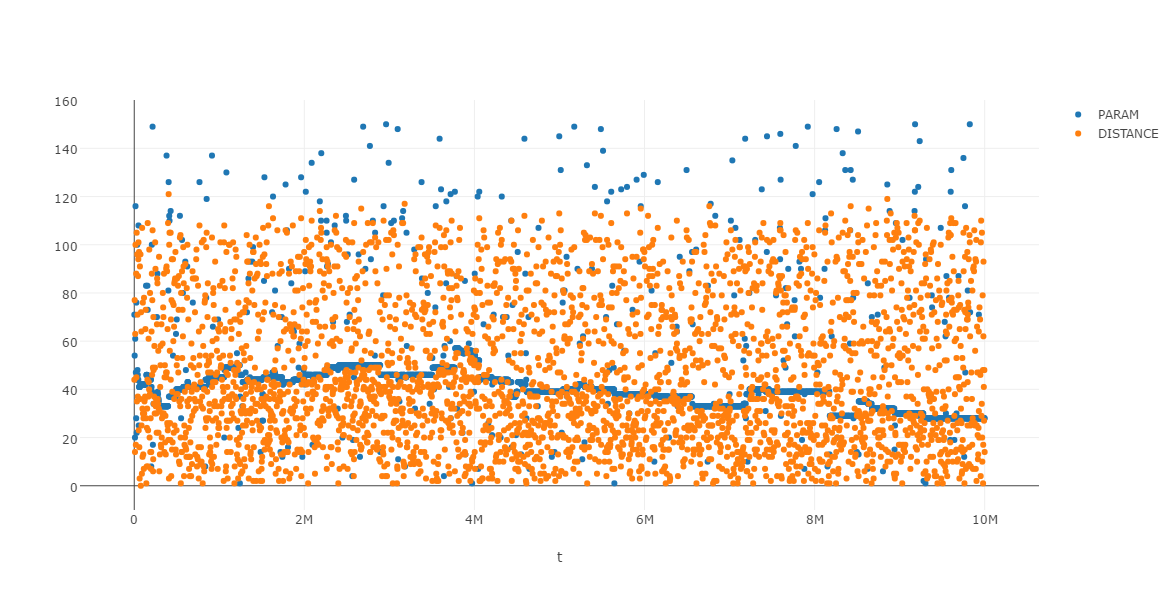
\includegraphics[width=0.8\textwidth]{analyse/SingleMutant/fixeddistance2.png}
	\caption{\emph{Fixed-Distance}-Heuristik bei 2 Autos pro Minute und einem lernenden Fahrer}\label{fig:ap_sm_fd_2}
\end{figure}
\begin{figure}[H]
	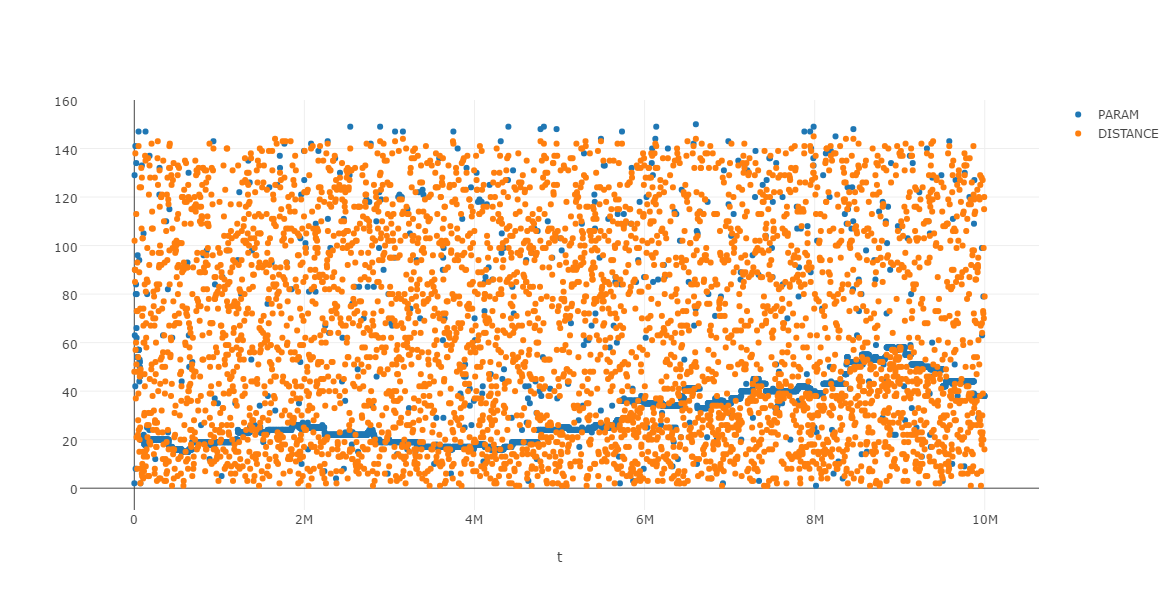
\includegraphics[width=0.8\textwidth]{analyse/SingleMutant/fixeddistance4.png}
	\caption{\emph{Fixed-Distance}-Heuristik bei 4 Autos pro Minute und einem lernenden Fahrer}\label{fig:ap_sm_fd_4}
\end{figure}
\begin{figure}[H]
	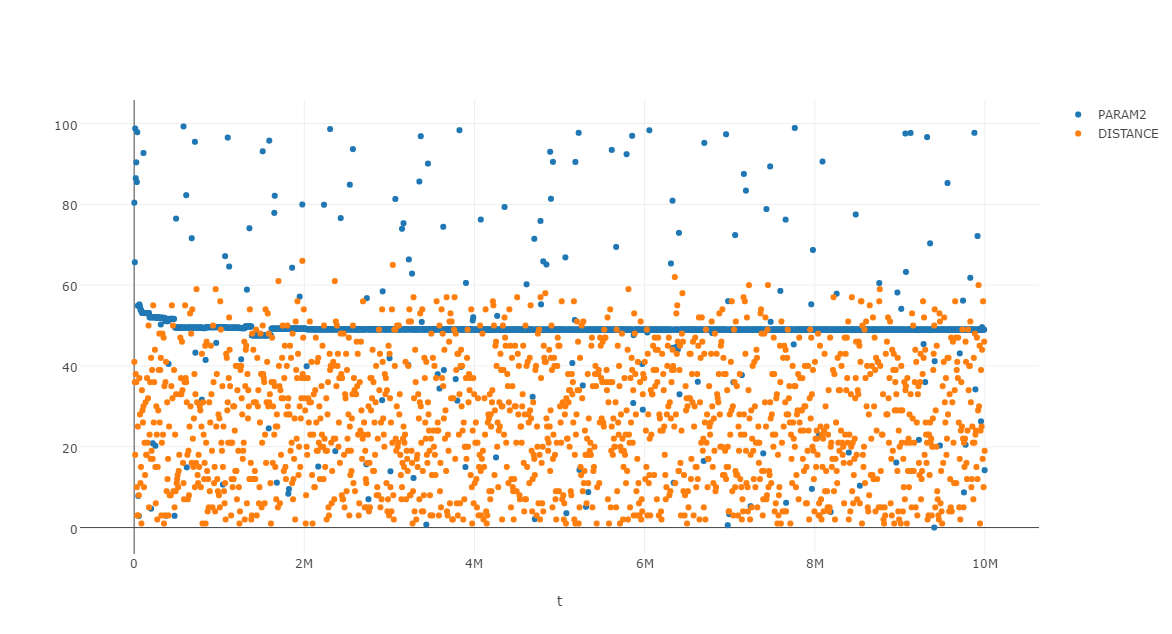
\includegraphics[width=0.8\textwidth]{analyse/SingleMutant/linopzt1.png}
	\caption{Schranke der \emph{Linear-Operator}-Heuristik bei 1 Auto pro Minute und einem lernenden Fahrer}\label{fig:ap_sm_loz_1}
\end{figure}
\begin{figure}[H]
	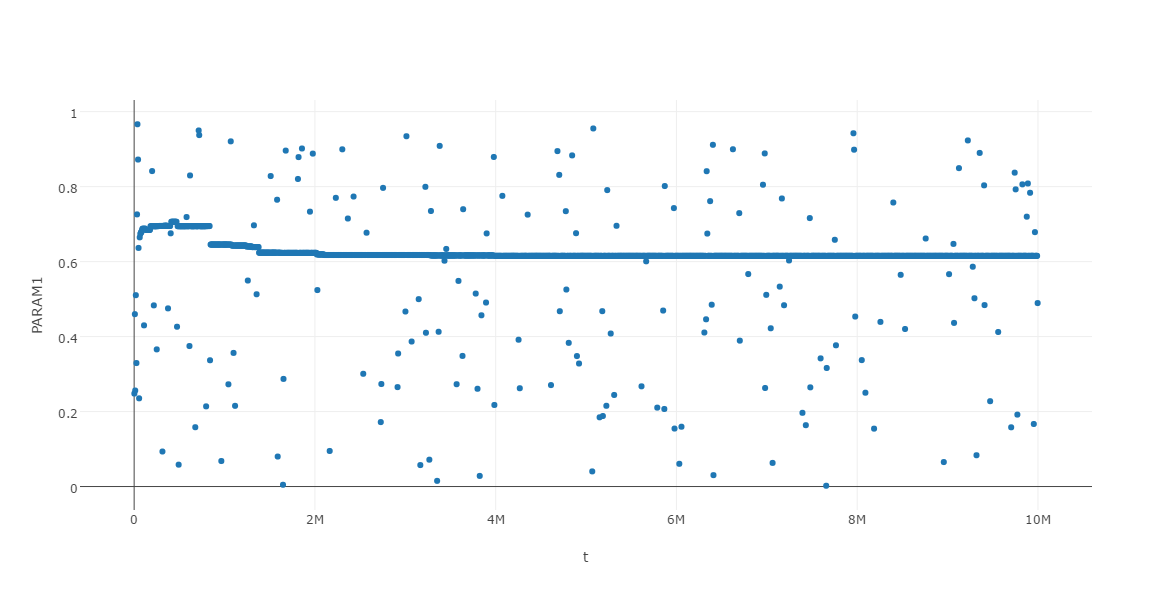
\includegraphics[width=0.8\textwidth]{analyse/SingleMutant/linopa1.png}
	\caption{Geschwindigkeit der \emph{Linear-Operator}-Heuristik bei 1 Auto pro Minute und einem lernenden Fahrer}\label{fig:ap_sm_loa_1}
\end{figure}
\begin{figure}[H]
	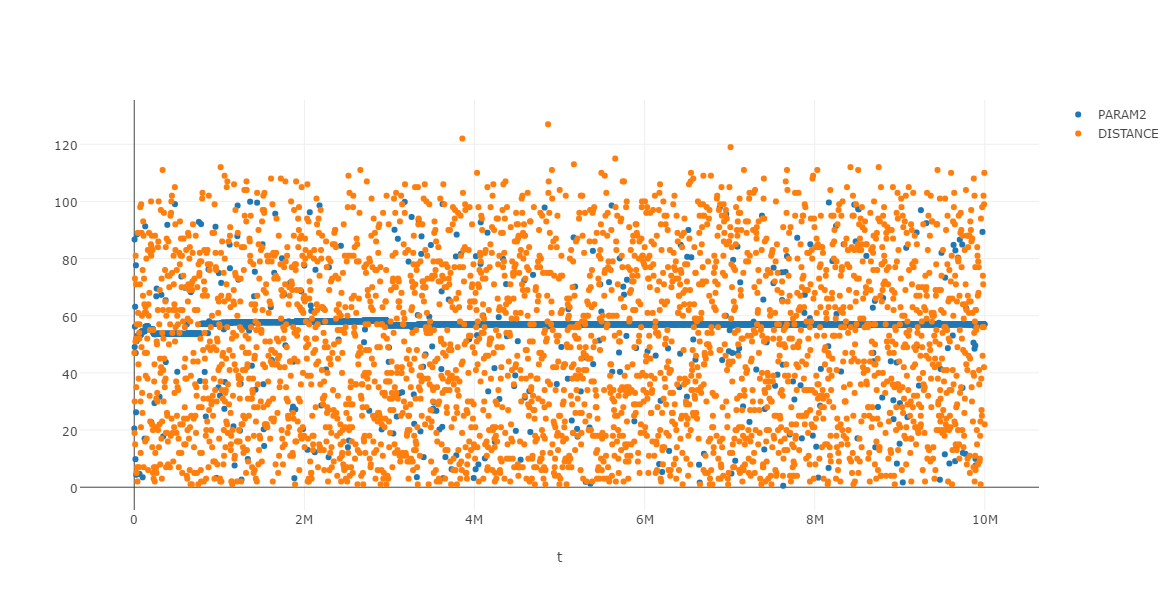
\includegraphics[width=0.8\textwidth]{analyse/SingleMutant/linopzt2.png}
	\caption{Schranke der \emph{Linear-Operator}-Heuristik bei 2 Autos pro Minute und einem lernenden Fahrer}\label{fig:ap_sm_loz_2}
\end{figure}
\begin{figure}[H]
	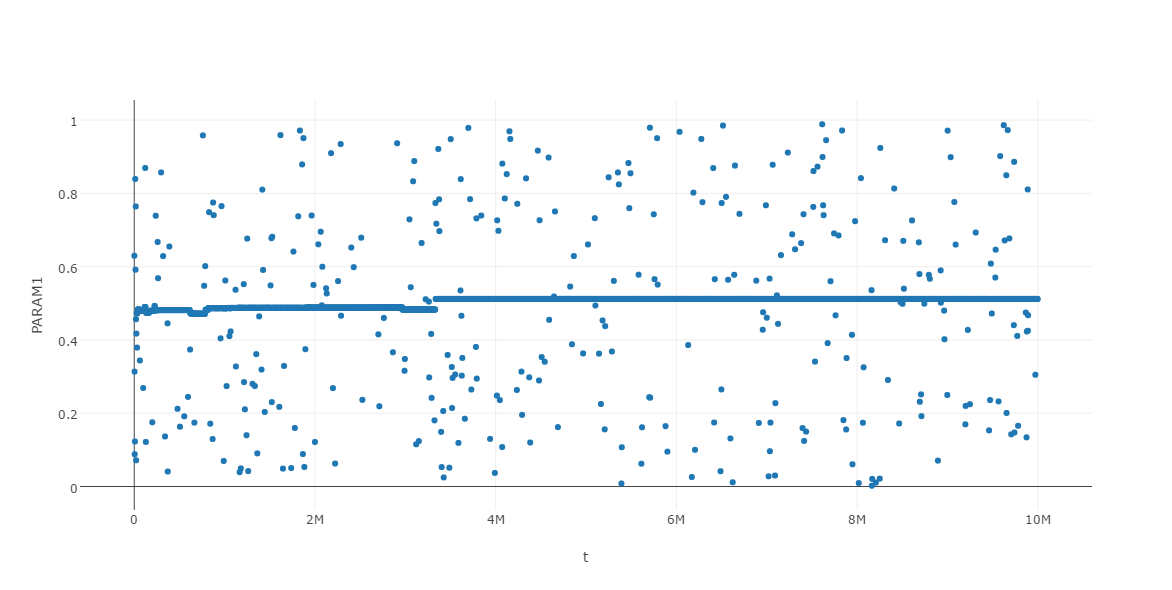
\includegraphics[width=0.8\textwidth]{analyse/SingleMutant/linopa2.png}
	\caption{Geschwindigkeit der \emph{Linear-Operator}-Heuristik bei 2 Autos pro Minute und einem lernenden Fahrer}\label{fig:ap_sm_loa_2}
\end{figure}
\begin{figure}[H]
	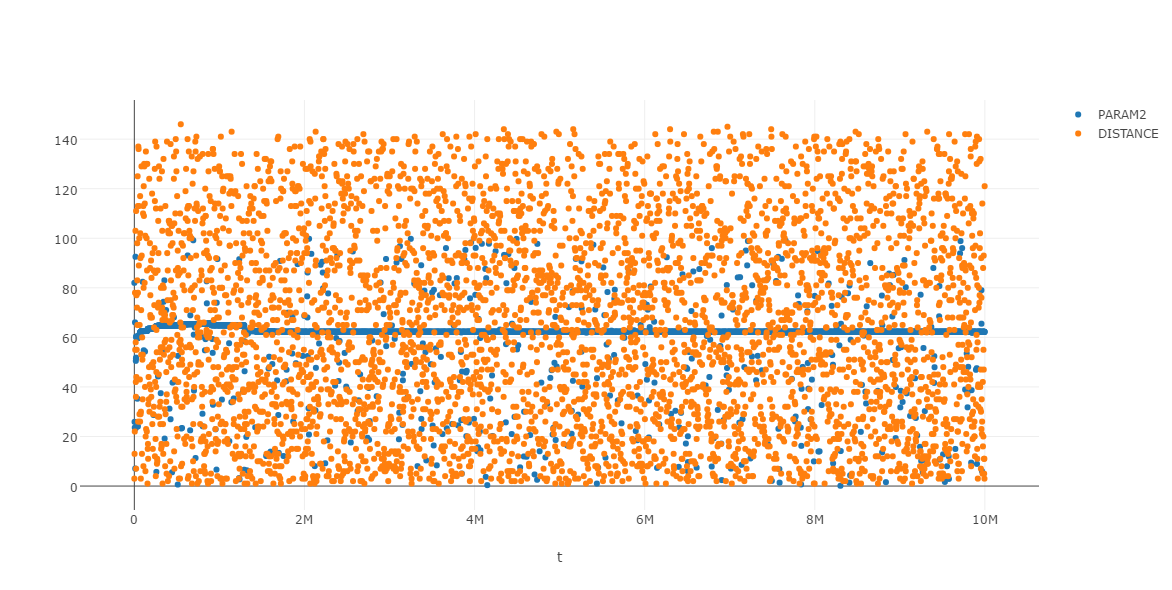
\includegraphics[width=0.8\textwidth]{analyse/SingleMutant/linopzt4.png}
	\caption{Schranke der \emph{Linear-Operator}-Heuristik bei 4 Autos pro Minute und einem lernenden Fahrer}\label{fig:ap_sm_loz_4}
\end{figure}
\begin{figure}[H]
	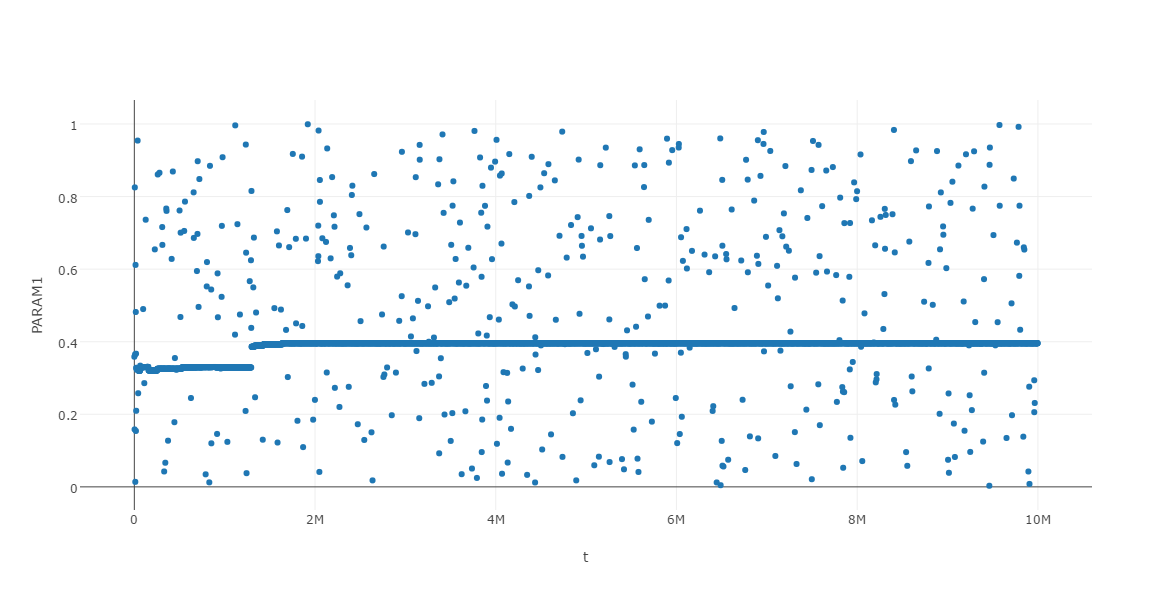
\includegraphics[width=0.8\textwidth]{analyse/SingleMutant/linopa4.png}
	\caption{Geschwindigkeit der \emph{Linear-Operator}-Heuristik bei 4 Autos pro Minute und einem lernenden Fahrer}\label{fig:ap_sm_loa_4}
\end{figure}
\begin{figure}[H]
	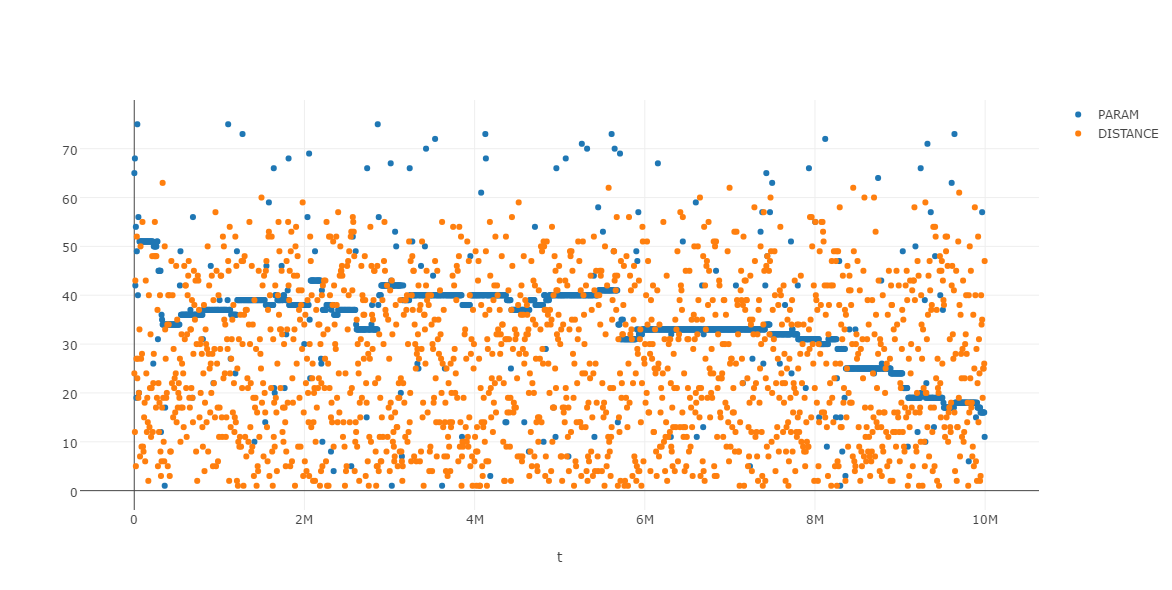
\includegraphics[width=0.8\textwidth]{analyse/SingleMutant/spacecount1.png}
	\caption{\emph{Space-Count}-Heuristik bei 1 Auto pro Minute und einem lernenden Fahrer}\label{fig:ap_sm_sc_1}
\end{figure}
\begin{figure}[H]
	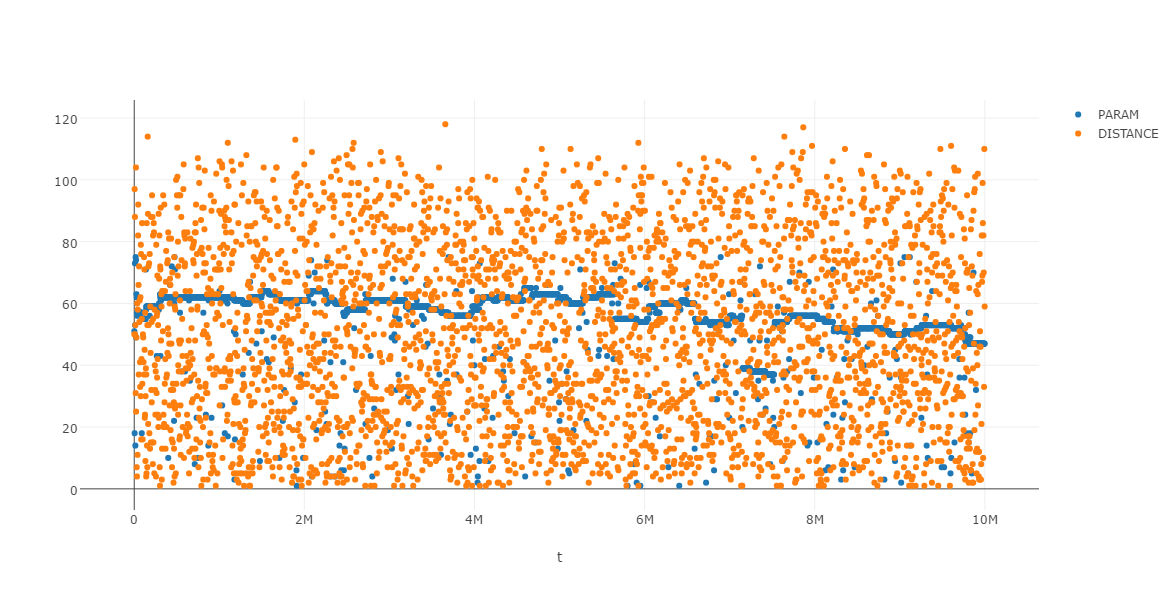
\includegraphics[width=0.8\textwidth]{analyse/SingleMutant/spacecount2.png}
	\caption{\emph{Space-Count}-Heuristik bei 2 Autos pro Minute und einem lernenden Fahrer}\label{fig:ap_sm_sc_2}
\end{figure}
\begin{figure}[H]
	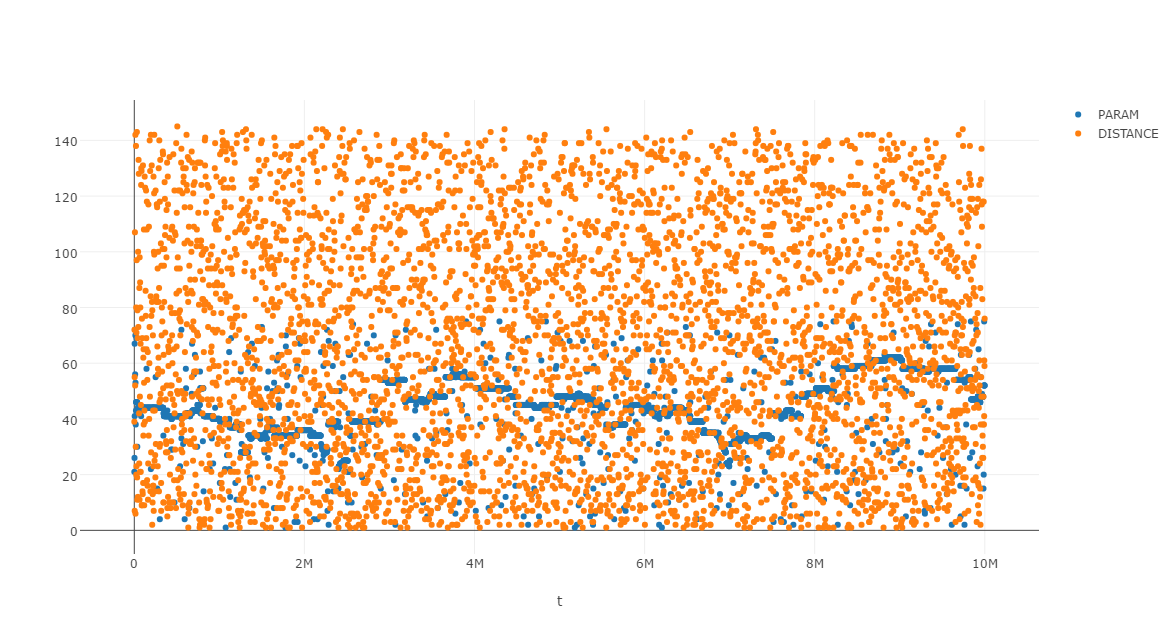
\includegraphics[width=0.8\textwidth]{analyse/SingleMutant/spacecount4.png}
	\caption{\emph{Space-Count}-Heuristik bei 4 Autos pro Minute und einem lernenden Fahrer}\label{fig:ap_sm_sc_4}
\end{figure}
\begin{figure}[H]
	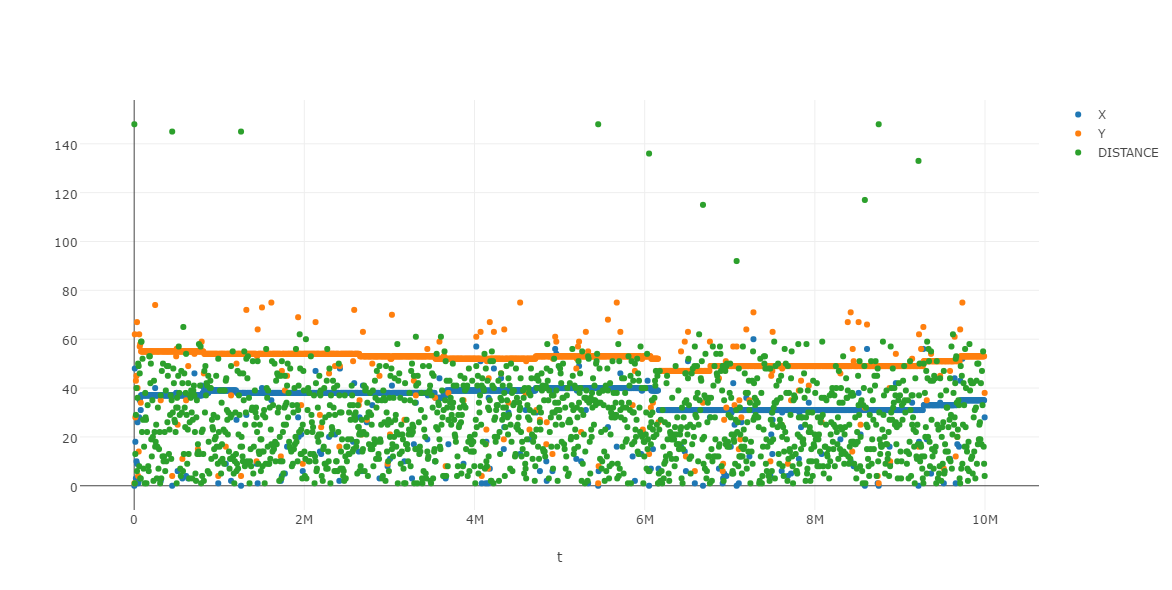
\includegraphics[width=0.8\textwidth]{analyse/SingleMutant/xy1.png}
	\caption{\emph{X-Out-Of-Y}-Heuristik bei 1 Auto pro Minute und einem lernenden Fahrer}\label{fig:ap_sm_xy_1}
\end{figure}
\begin{figure}[H]
	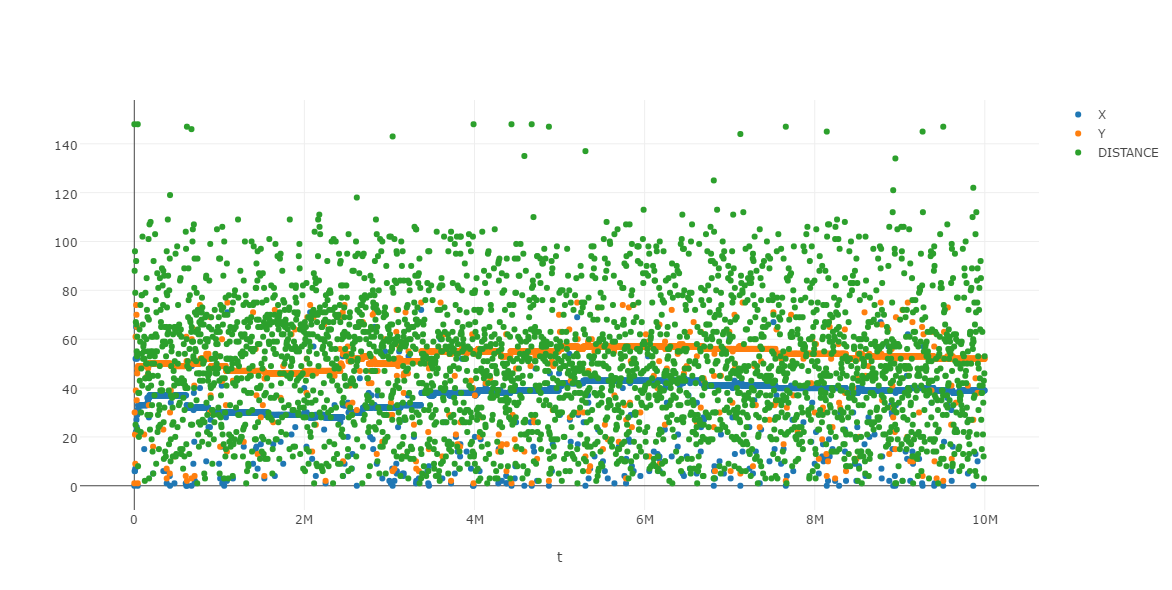
\includegraphics[width=0.8\textwidth]{analyse/SingleMutant/xy2.png}
	\caption{\emph{X-Out-Of-Y}-Heuristik bei 2 Autos pro Minute und einem lernenden Fahrer}\label{fig:ap_sm_xy_2}
\end{figure}
\begin{figure}[H]
	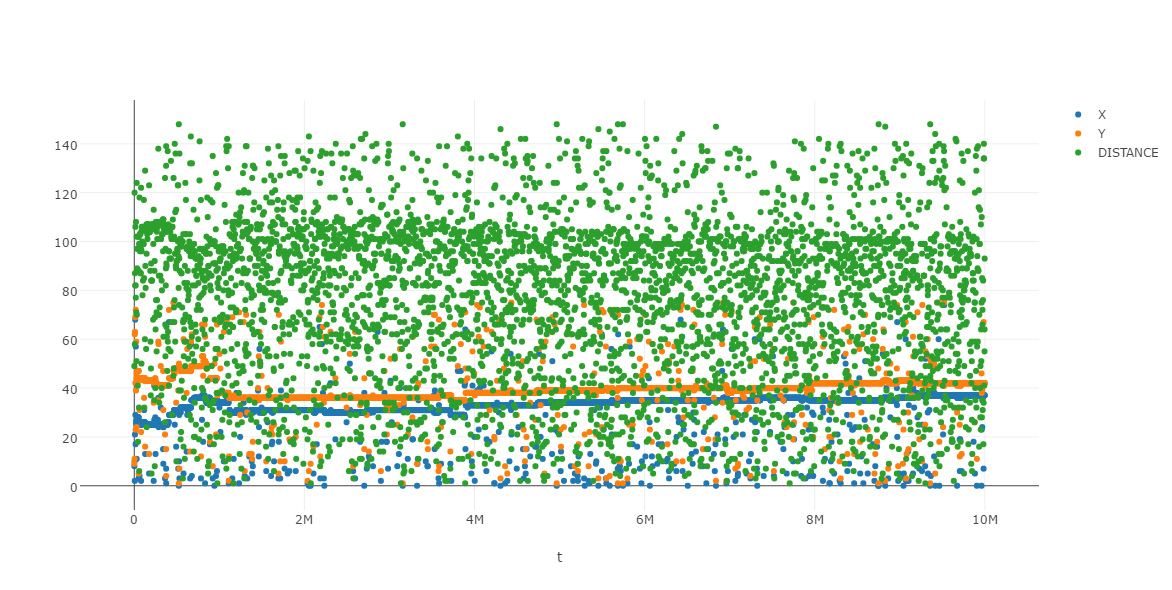
\includegraphics[width=0.8\textwidth]{analyse/SingleMutant/xy4.png}
	\caption{\emph{X-Out-Of-Y}-Heuristik bei 4 Autos pro Minute und einem lernenden Fahrer}\label{fig:ap_sm_xy_4}
\end{figure}

\subsubsection*{$20\%$ lernende Fahrer}
Im Gegensatz zum vorherigen Abschnitt sind die Heuristiken nun nach der durchgeführten Simulation sortiert.
\begin{figure}[H]
	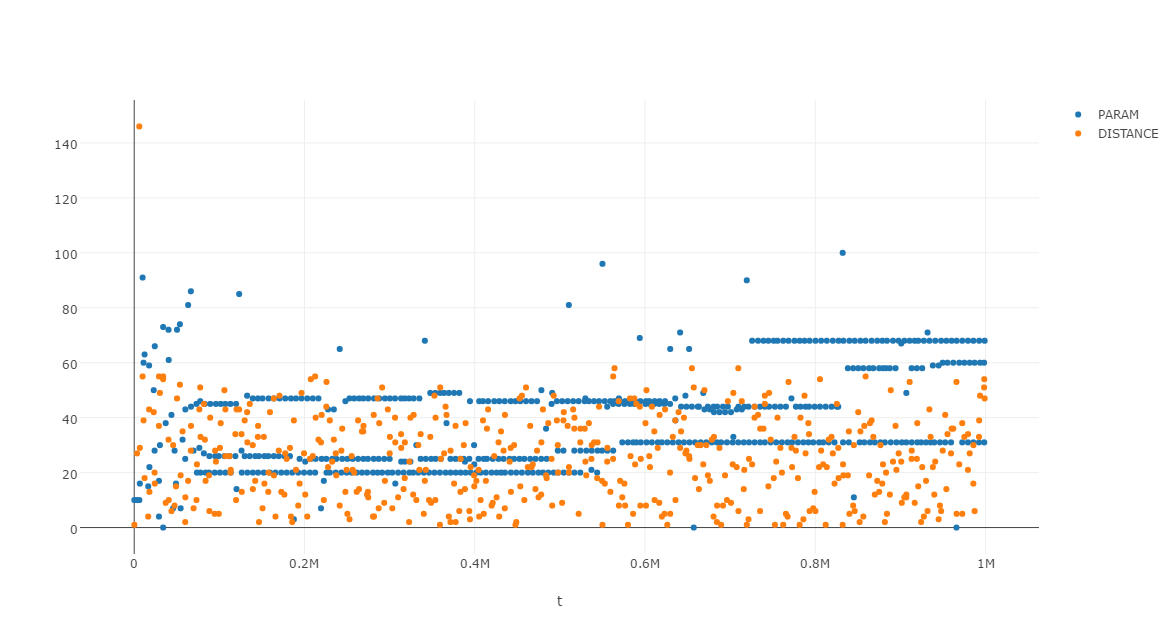
\includegraphics[width=0.8\textwidth]{analyse/SomeMutants/1pm/block1some.png}
	\caption{\emph{Block-Count}-Heuristik bei 1 Auto pro Minute und $20\%$ lernenden Fahrern}\label{fig:ap_pm_bs_1}
\end{figure}
\begin{figure}[H]
	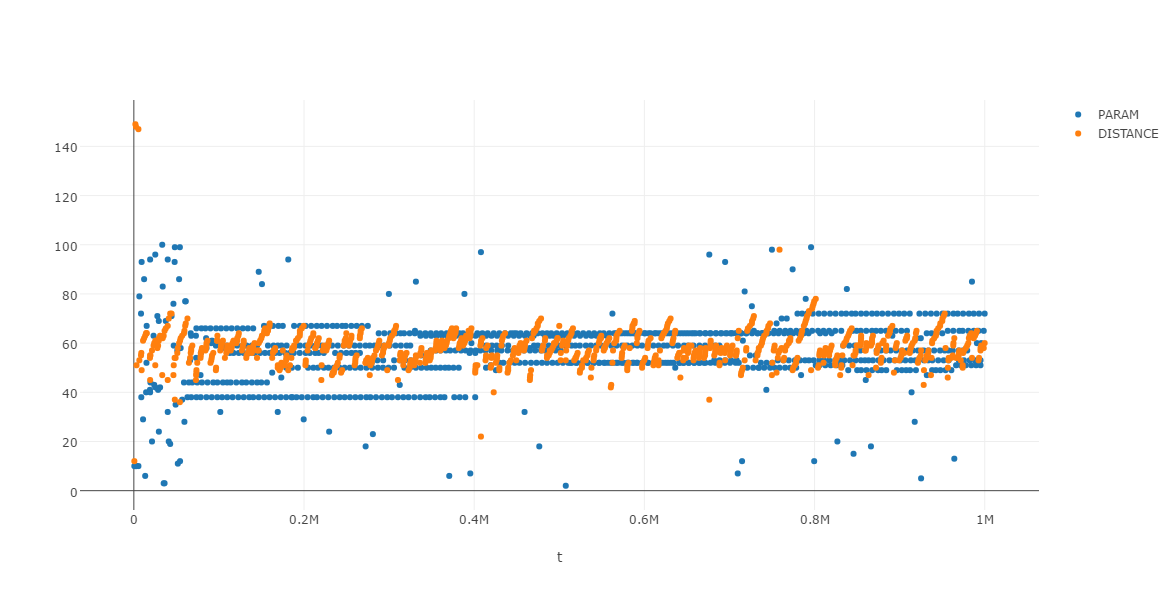
\includegraphics[width=0.8\textwidth]{analyse/SomeMutants/1pm/car1some.png}
	\caption{\emph{Car-Count}-Heuristik bei 1 Auto pro Minute und $20\%$ lernenden Fahrern}\label{fig:ap_pm_cc_1}
\end{figure}
\begin{figure}[H]
	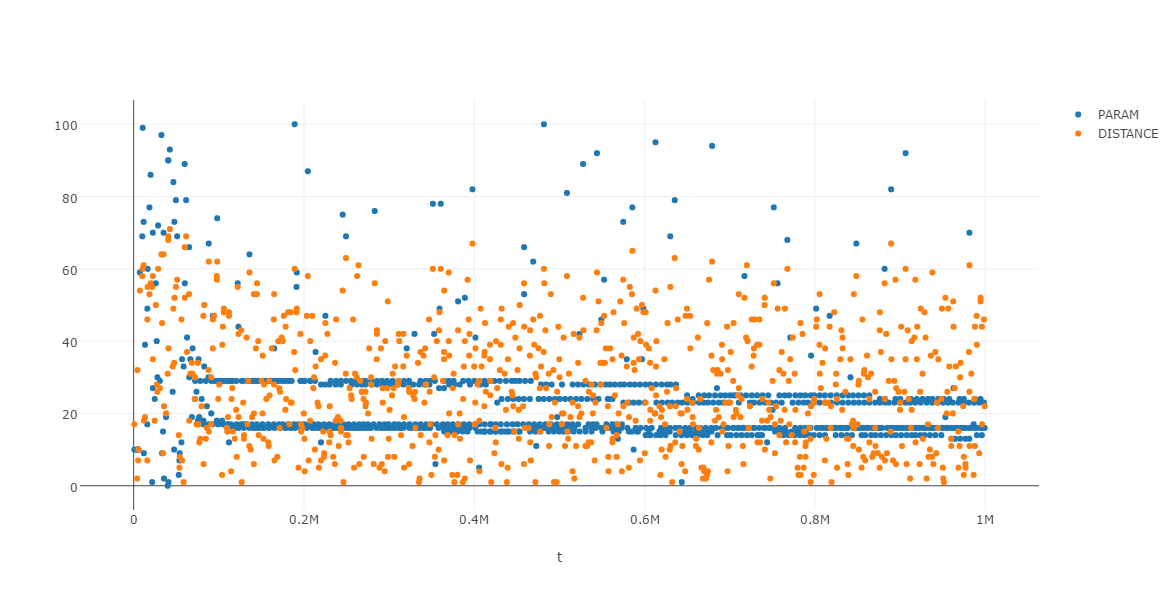
\includegraphics[width=0.8\textwidth]{analyse/SomeMutants/1pm/fixed1some.png}
	\caption{\emph{Fixed-Distance}-Heuristik bei 1 Auto pro Minute und $20\%$ lernenden Fahrern}\label{fig:ap_pm_fd_1}
\end{figure}
\begin{figure}[H]
	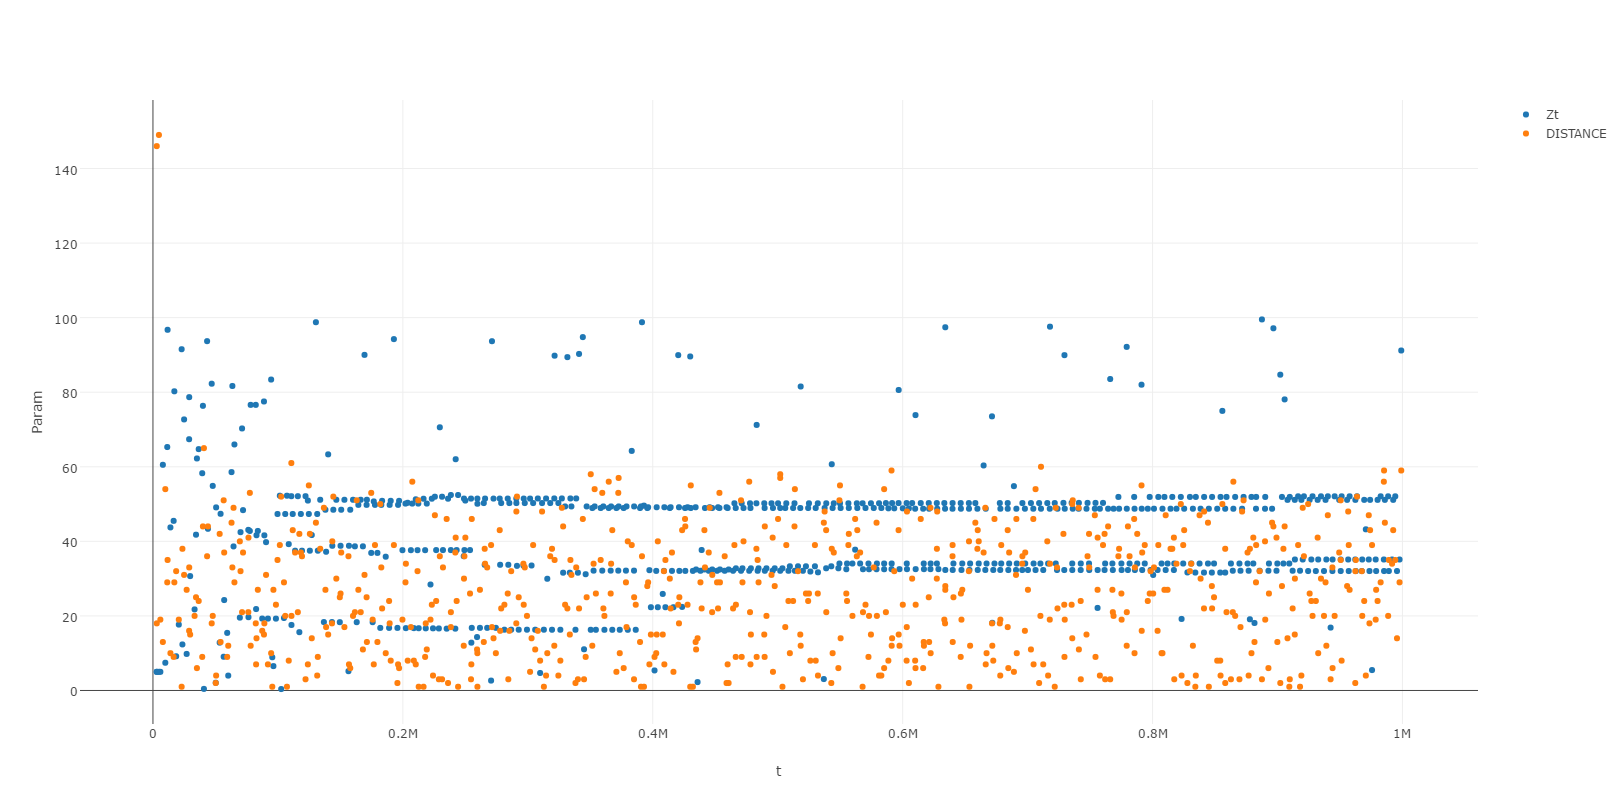
\includegraphics[width=0.8\textwidth]{analyse/SomeMutants/1pm/linop.png}
	\caption{Schranke der \emph{Linear-Operator}-Heuristik bei 1 Auto pro Minute und $20\%$ lernenden Fahrern}\label{fig:ap_pm_loz_1}
\end{figure}
\begin{figure}[H]
	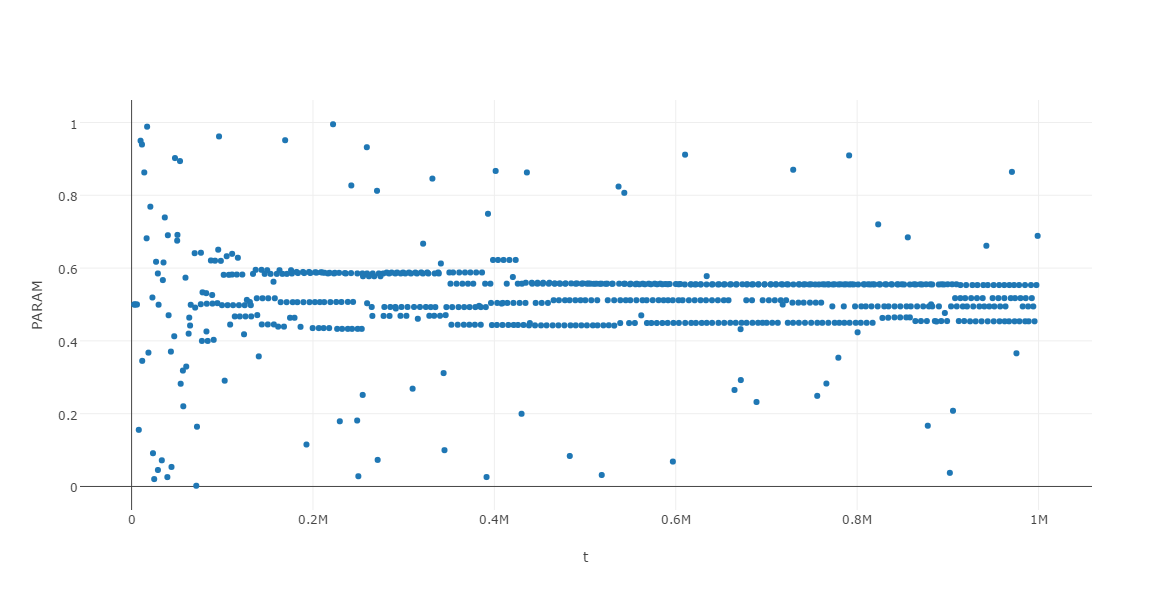
\includegraphics[width=0.8\textwidth]{analyse/SomeMutants/1pm/linopa1some.png}
	\caption{Geschwindigkeit der \emph{Linear-Operator}-Heuristik bei 1 Auto pro Minute und $20\%$ lernenden Fahrern}\label{fig:ap_pm_loa_1}
\end{figure}
\begin{figure}[H]
	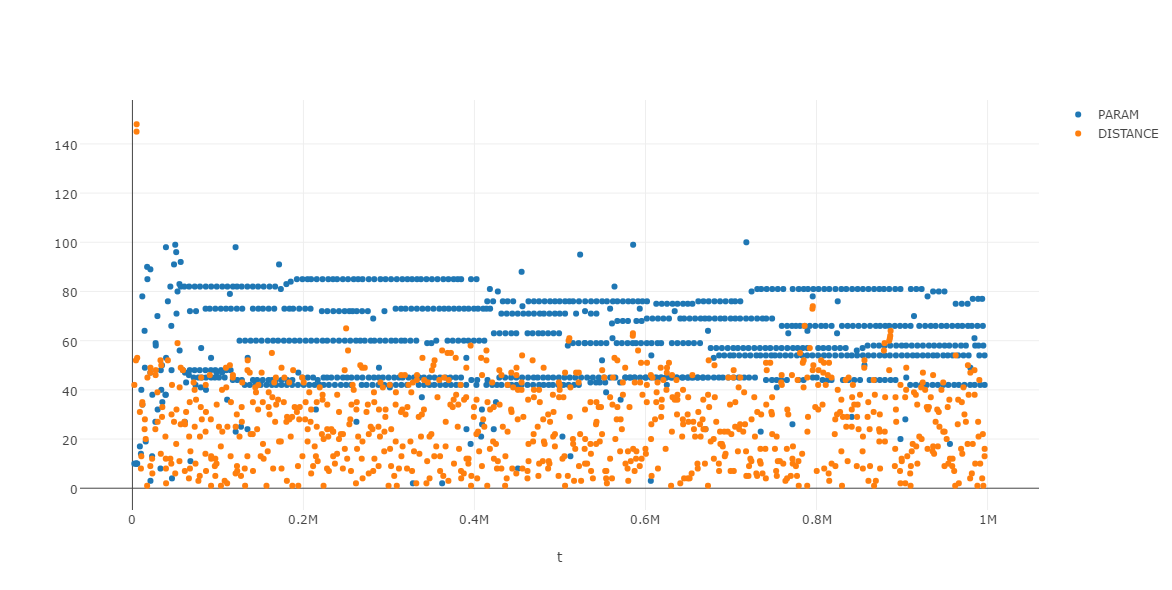
\includegraphics[width=0.8\textwidth]{analyse/SomeMutants/1pm/space1some.png}
	\caption{\emph{Space-Count}-Heuristik bei 1 Auto pro Minute und $20\%$ lernenden Fahrern}\label{fig:ap_pm_sc_1}
\end{figure}
\begin{figure}[H]
	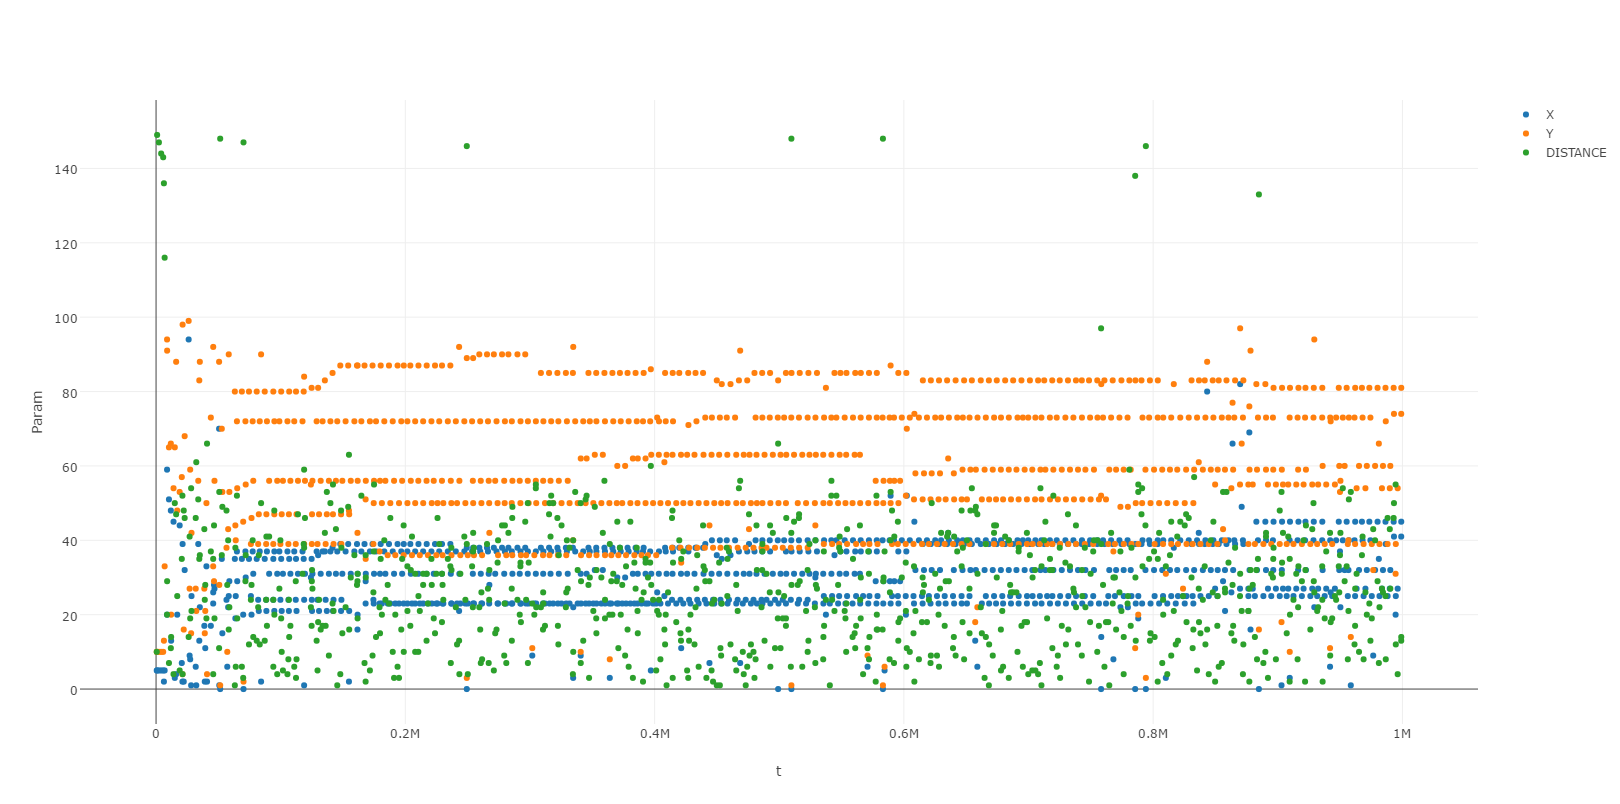
\includegraphics[width=0.8\textwidth]{analyse/SomeMutants/1pm/xy.png}
	\caption{\emph{X-Out-Of-Y}-Heuristik bei 1 Auto pro Minute und $20\%$ lernenden Fahrern}\label{fig:ap_pm_xy_1}
\end{figure}
\begin{figure}[H]
	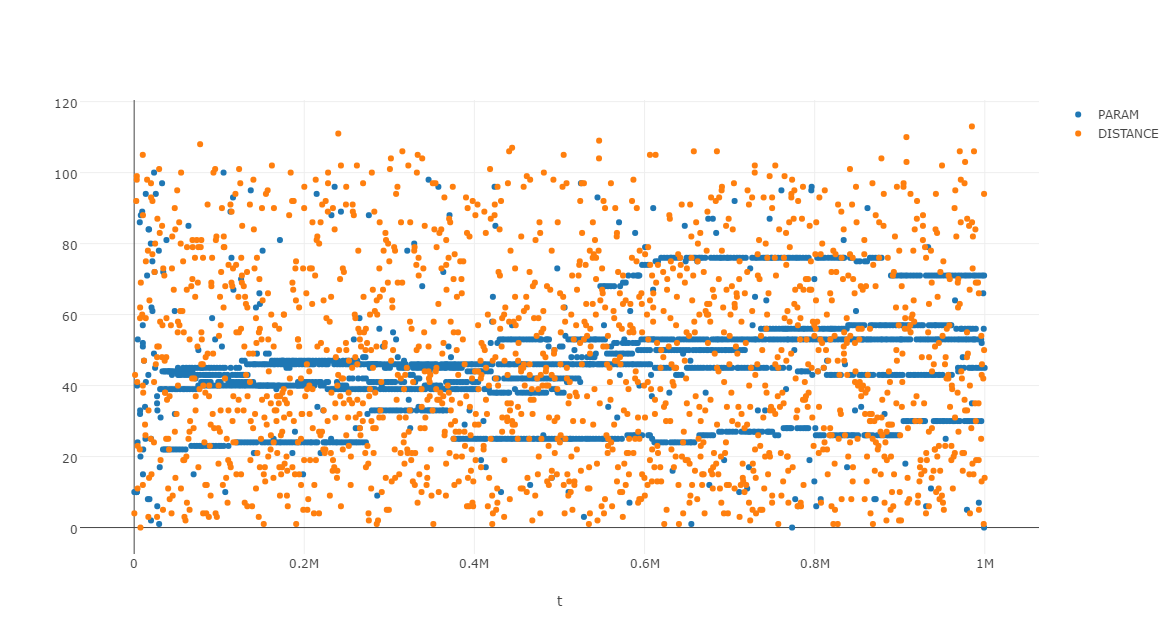
\includegraphics[width=0.8\textwidth]{analyse/SomeMutants/2pm/block2some.png}
	\caption{\emph{Block-Count}-Heuristik bei 2 Autos pro Minute und $20\%$ lernenden Fahrern}\label{fig:ap_pm_bs_2}
\end{figure}
\begin{figure}[H]
	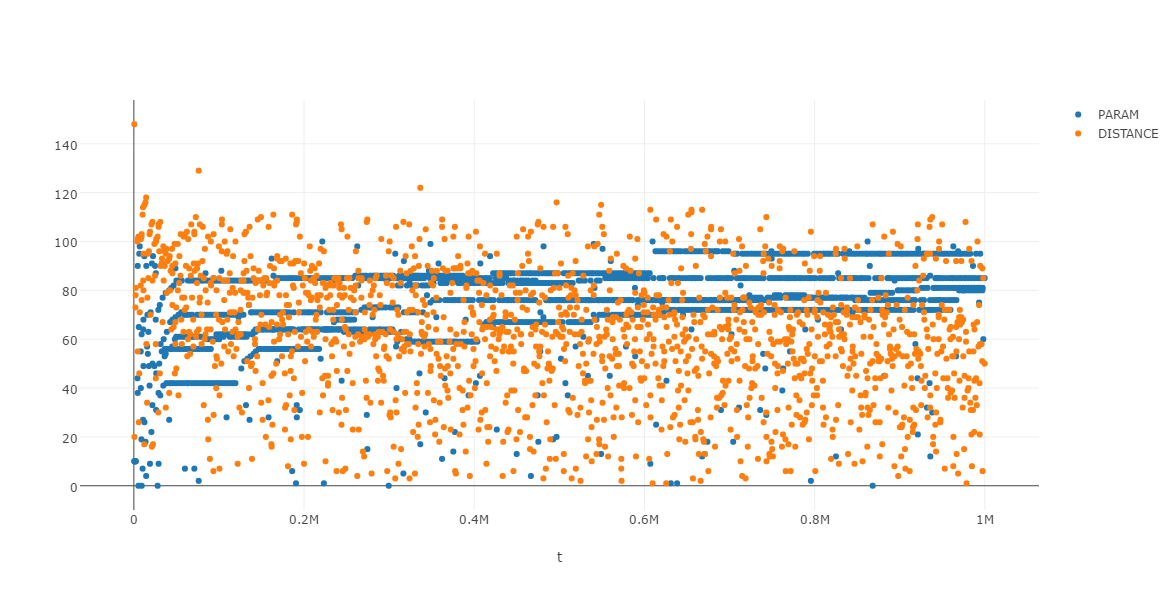
\includegraphics[width=0.8\textwidth]{analyse/SomeMutants/2pm/car2some.png}
	\caption{\emph{Car-Count}-Heuristik bei 2 Autos pro Minute und $20\%$ lernenden Fahrern}\label{fig:ap_pm_cc_2}
\end{figure}
\begin{figure}[H]
	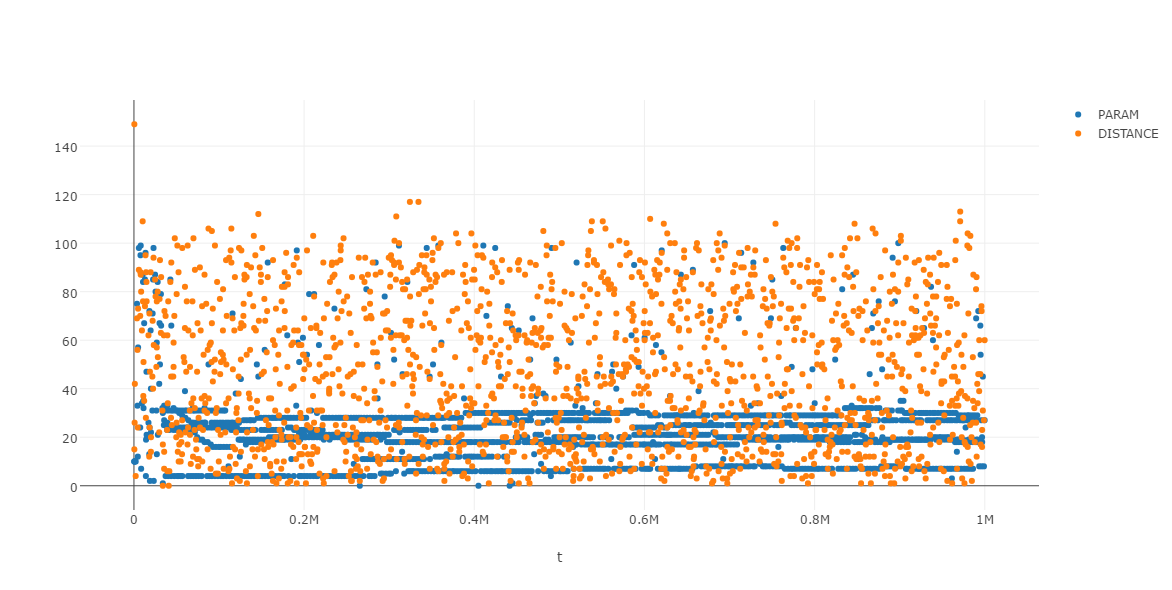
\includegraphics[width=0.8\textwidth]{analyse/SomeMutants/2pm/fixed2some.png}
	\caption{\emph{Fixed-Distance}-Heuristik bei 2 Autos pro Minute und $20\%$ lernenden Fahrern}\label{fig:ap_pm_fd_2}
\end{figure}
\begin{figure}[H]
	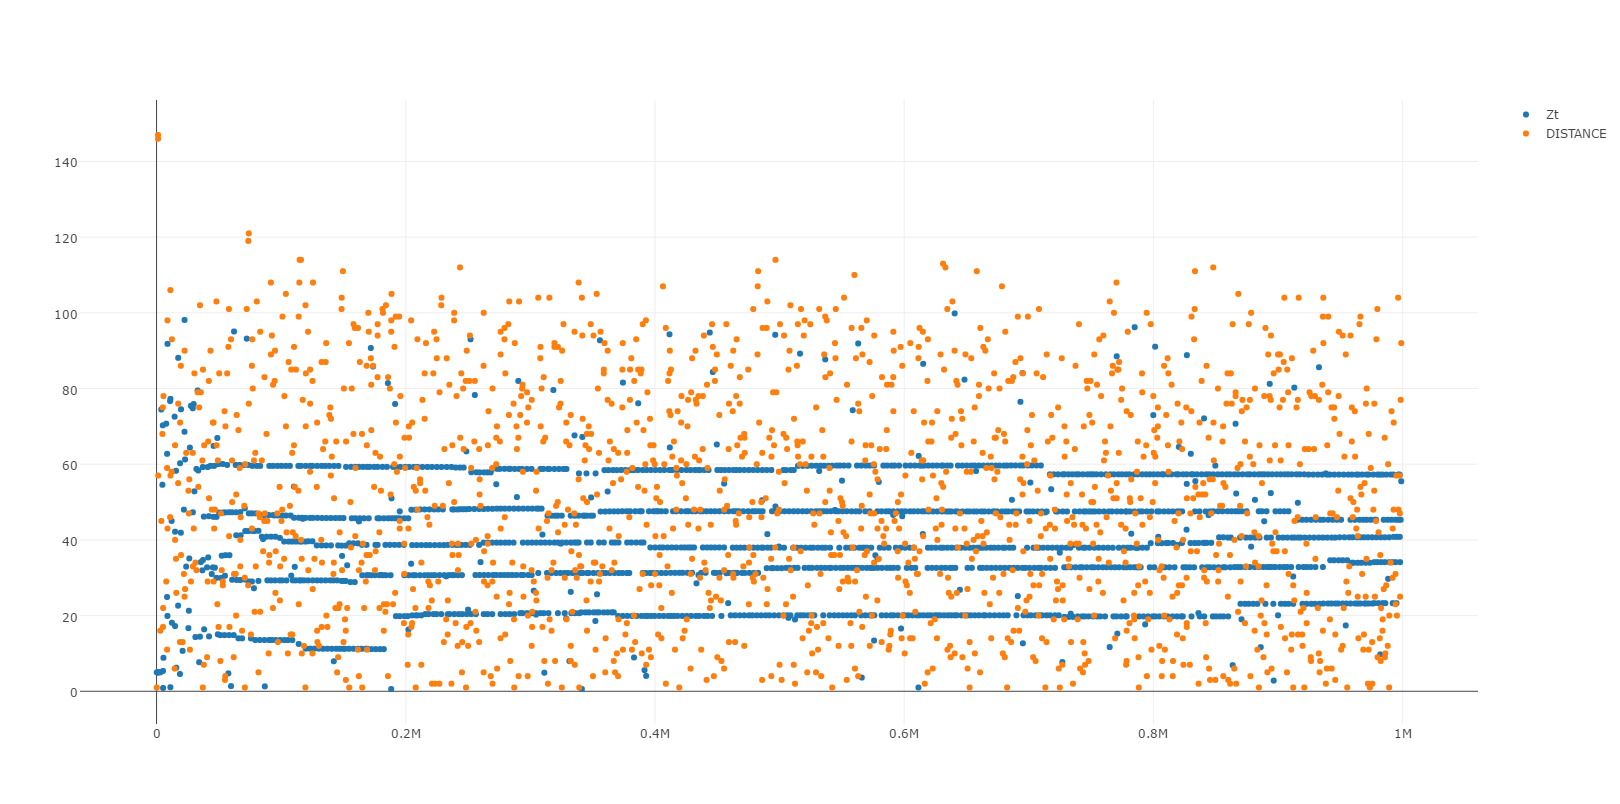
\includegraphics[width=0.8\textwidth]{analyse/SomeMutants/2pm/linop.png}
	\caption{Schranke der \emph{Linear-Operator}-Heuristik bei 2 Autos pro Minute und $20\%$ lernenden Fahrern}\label{fig:ap_pm_loz_2}
\end{figure}
\begin{figure}[H]
	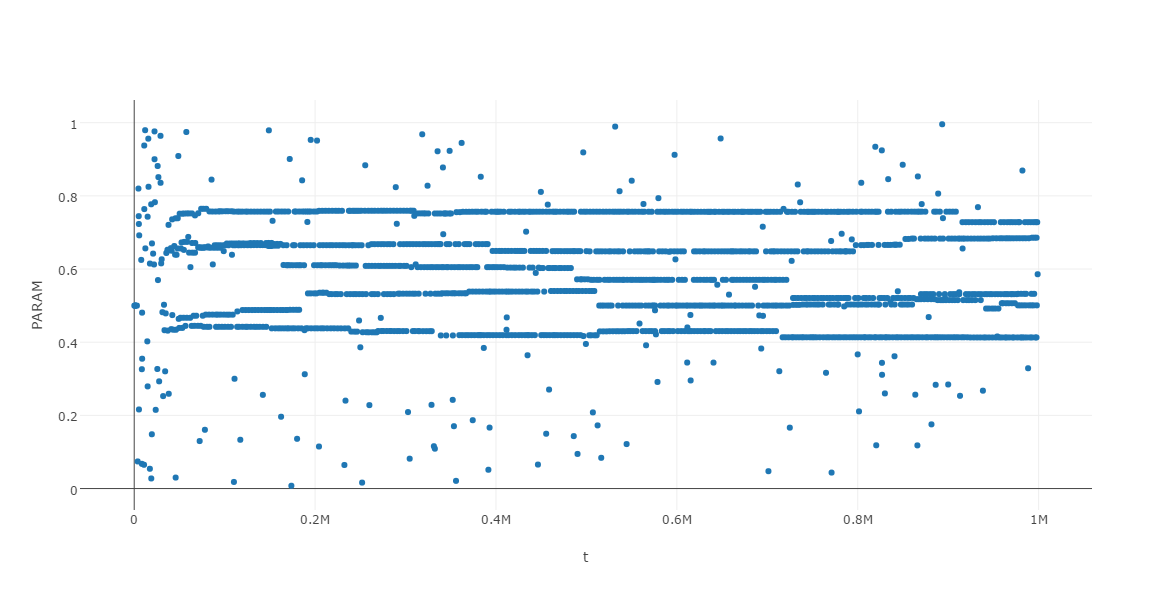
\includegraphics[width=0.8\textwidth]{analyse/SomeMutants/2pm/linopa2some.png}
	\caption{Geschwindigkeit der \emph{Linear-Operator}-Heuristik bei 2 Autos pro Minute und $20\%$ lernenden Fahrern}\label{fig:ap_pm_loa_2}
\end{figure}
\begin{figure}[H]
	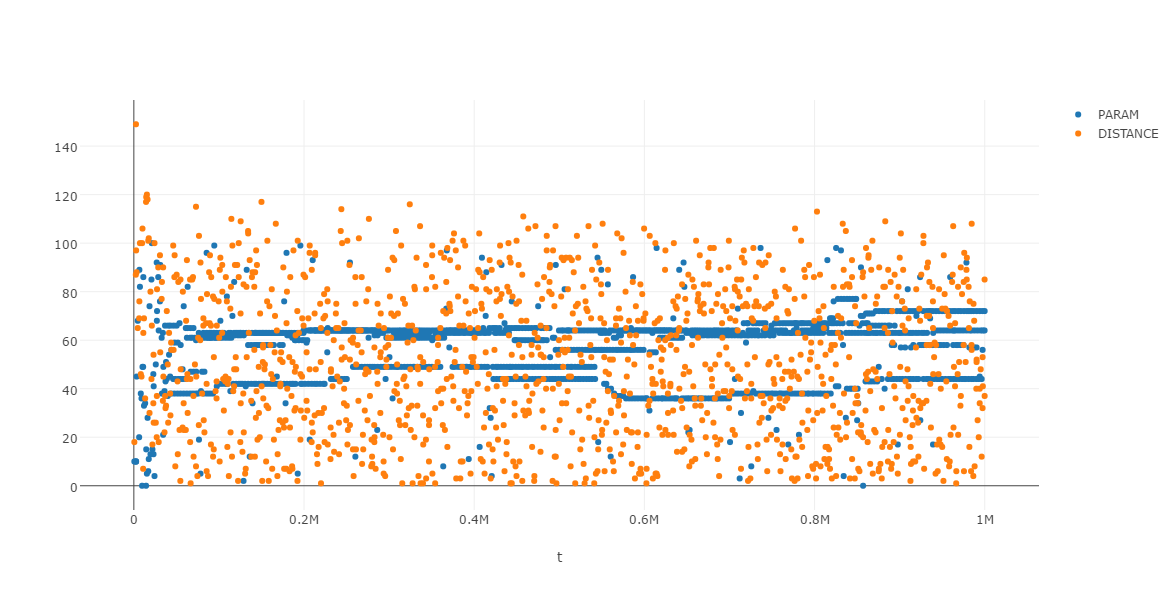
\includegraphics[width=0.8\textwidth]{analyse/SomeMutants/2pm/space2some.png}
	\caption{\emph{Space-Count}-Heuristik bei 2 Autos pro Minute und $20\%$ lernenden Fahrern}\label{fig:ap_pm_sc_2}
\end{figure}
\begin{figure}[H]
	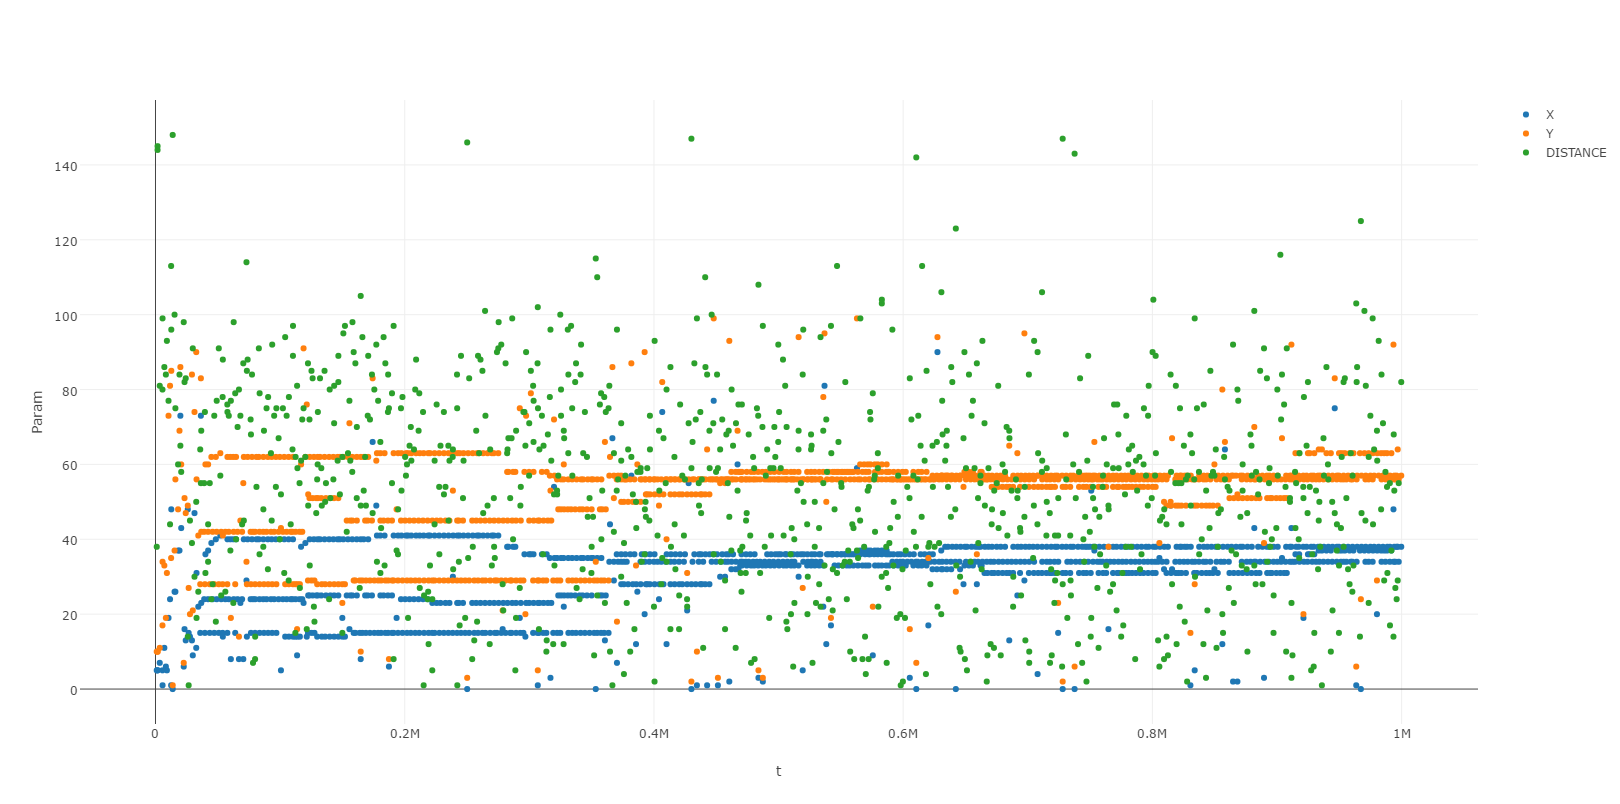
\includegraphics[width=0.8\textwidth]{analyse/SomeMutants/2pm/xy.png}
	\caption{\emph{X-Out-Of-Y}-Heuristik bei 2 Autos pro Minute und $20\%$ lernenden Fahrern}\label{fig:ap_pm_xy_2}
\end{figure}
\begin{figure}[H]
	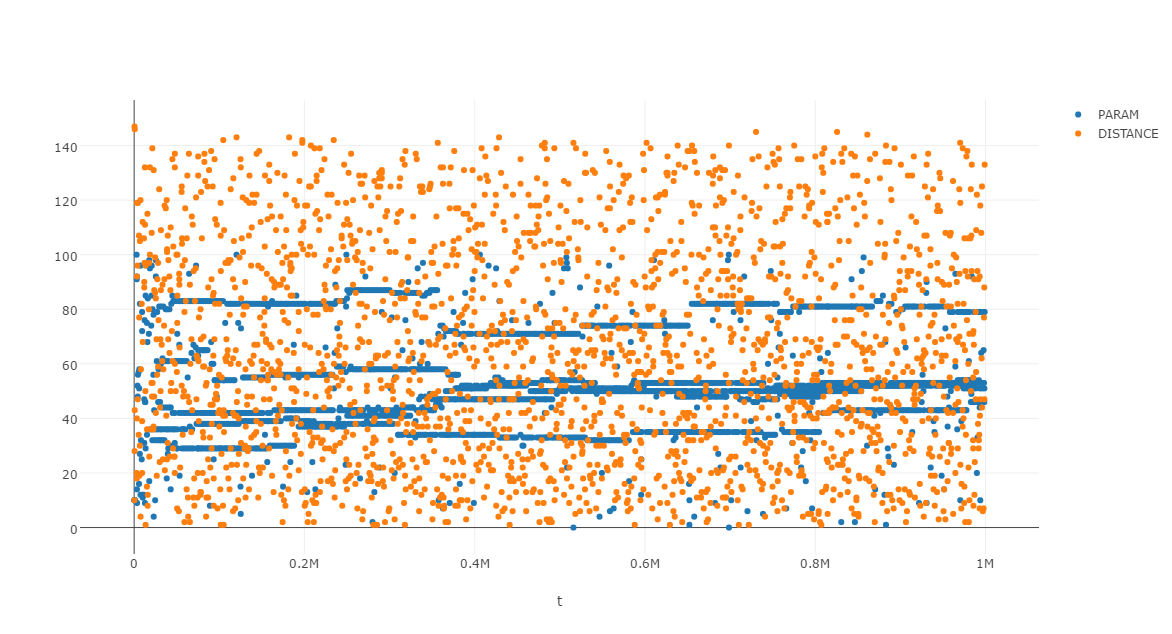
\includegraphics[width=0.8\textwidth]{analyse/SomeMutants/4pm/block4some.png}
	\caption{\emph{Block-Count}-Heuristik bei 4 Autos pro Minute und $20\%$ lernenden Fahrern}\label{fig:ap_pm_bs_4}
\end{figure}
\begin{figure}[H]
	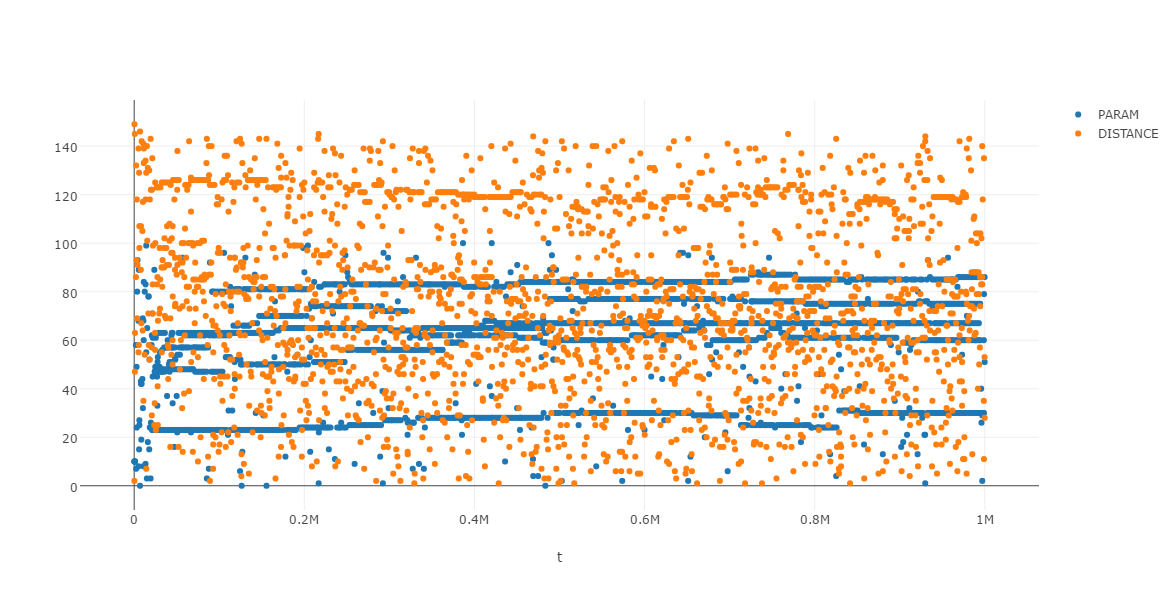
\includegraphics[width=0.8\textwidth]{analyse/SomeMutants/4pm/car4some.png}
	\caption{\emph{Car-Count}-Heuristik bei 4 Autos pro Minute und $20\%$ lernenden Fahrern}\label{fig:ap_pm_cc_4}
\end{figure}
\begin{figure}[H]
	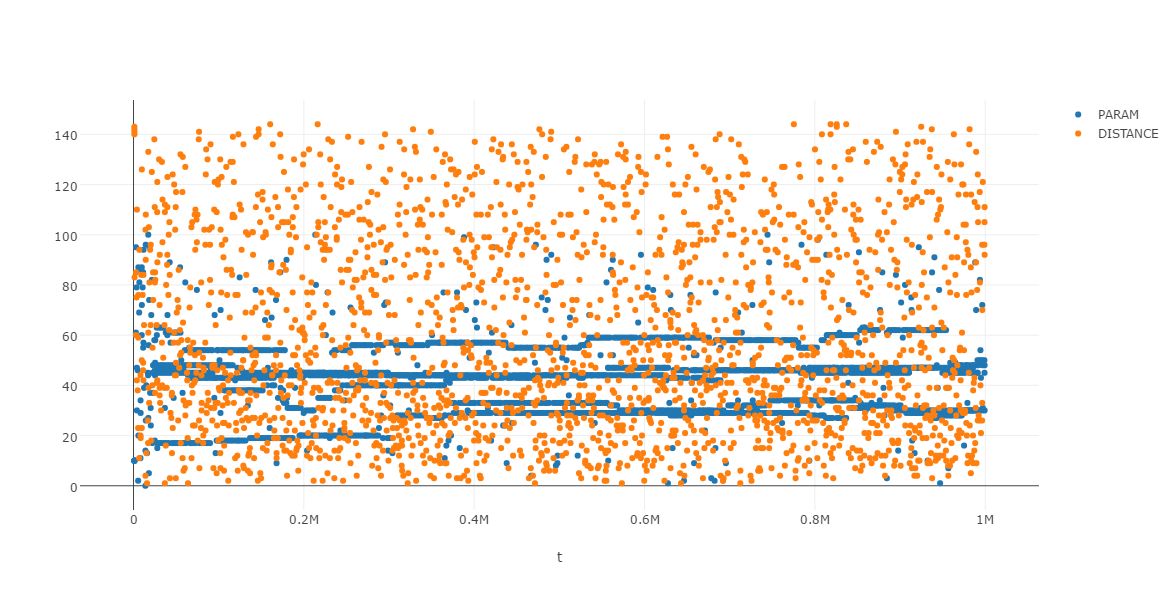
\includegraphics[width=0.8\textwidth]{analyse/SomeMutants/4pm/fixed4some.png}
	\caption{\emph{Fixed-Distance}-Heuristik bei 4 Autos pro Minute und $20\%$ lernenden Fahrern}\label{fig:ap_pm_fd_4}
\end{figure}
\begin{figure}[H]
	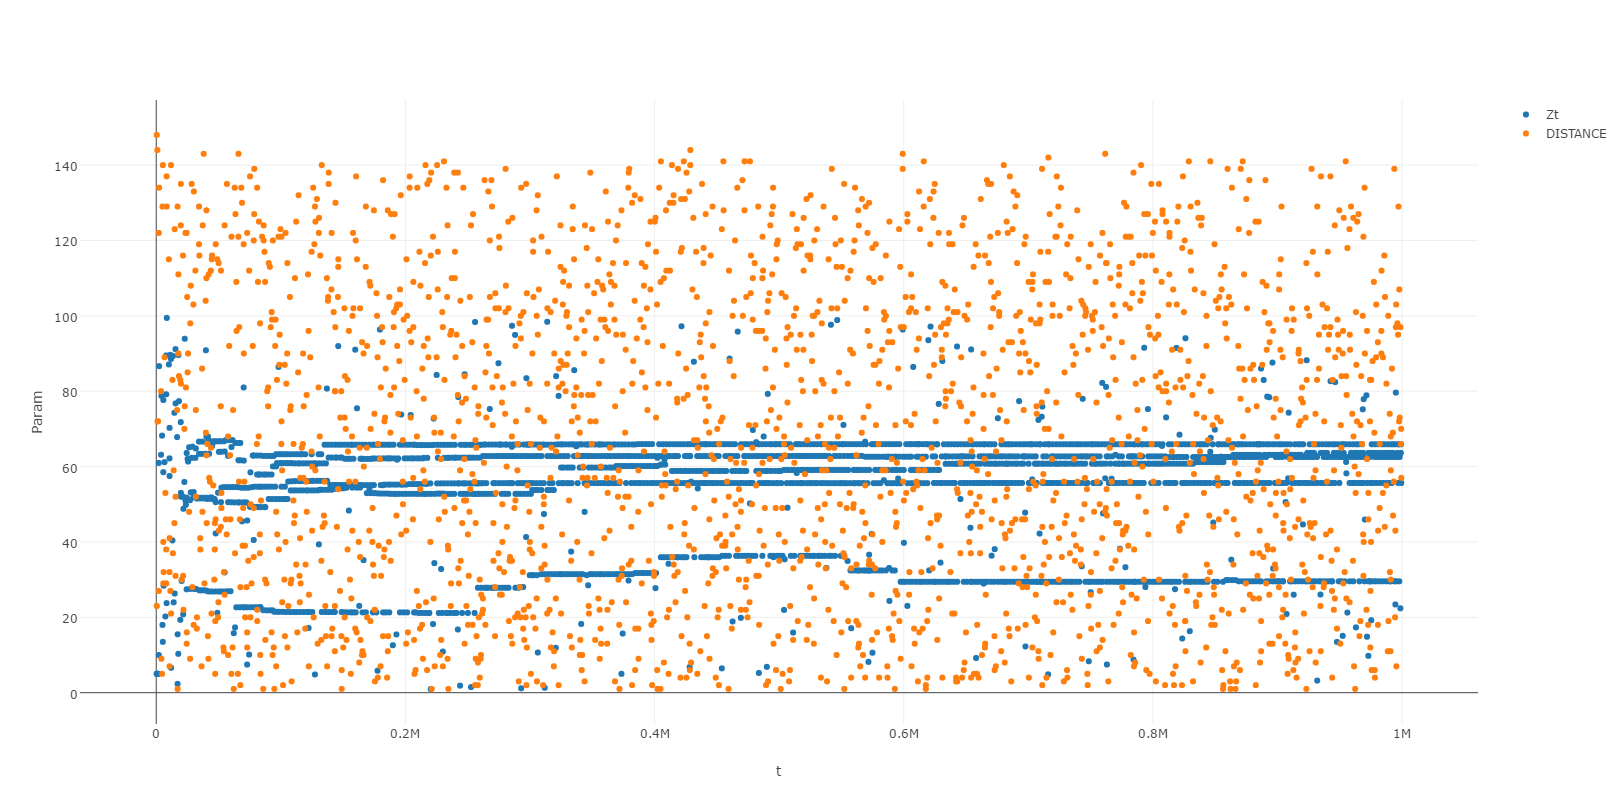
\includegraphics[width=0.8\textwidth]{analyse/SomeMutants/4pm/linop.png}
	\caption{Schranke der \emph{Linear-Operator}-Heuristik bei 4 Autos pro Minute und $20\%$ lernenden Fahrern}\label{fig:ap_pm_loz_4}
\end{figure}
\begin{figure}[H]
	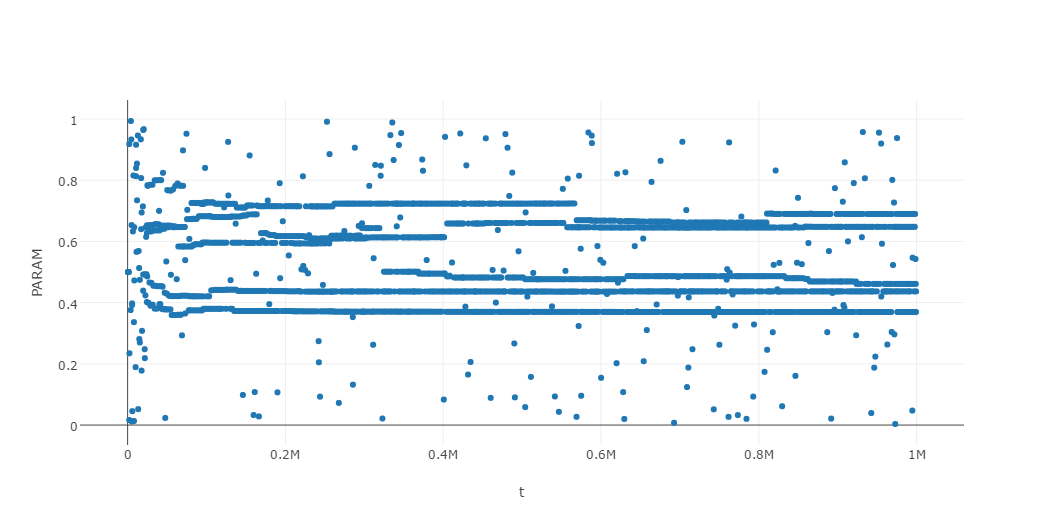
\includegraphics[width=0.8\textwidth]{analyse/SomeMutants/4pm/linopa4some.png}
	\caption{Geschwindigkeit der \emph{Linear-Operator}-Heuristik bei 4 Autos pro Minute und $20\%$ lernenden Fahrern}\label{fig:ap_pm_loa_4}
\end{figure}
\begin{figure}[H]
	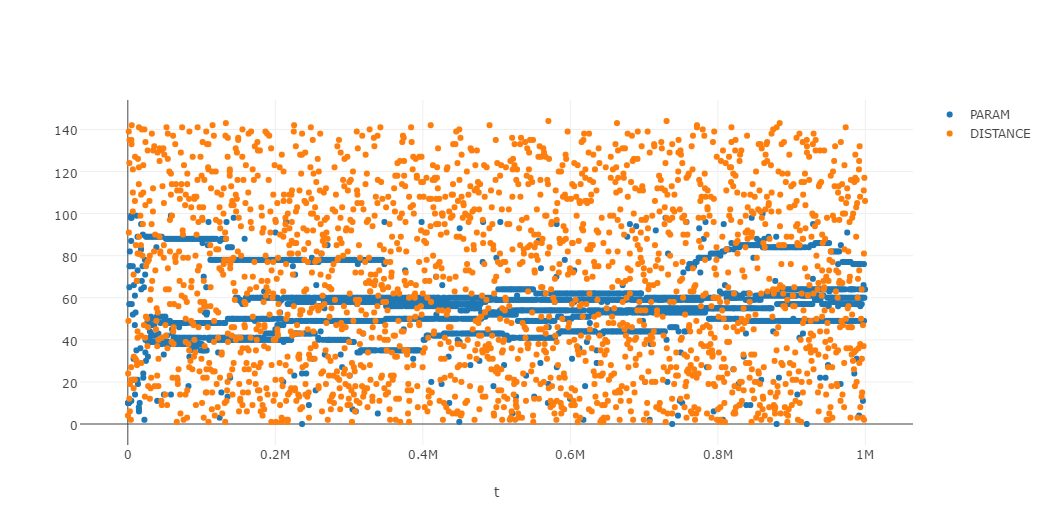
\includegraphics[width=0.8\textwidth]{analyse/SomeMutants/4pm/space4some.png}
	\caption{\emph{Space-Count}-Heuristik bei 4 Autos pro Minute und $20\%$ lernenden Fahrern}\label{fig:ap_pm_sc_4}
\end{figure}
\begin{figure}[H]
	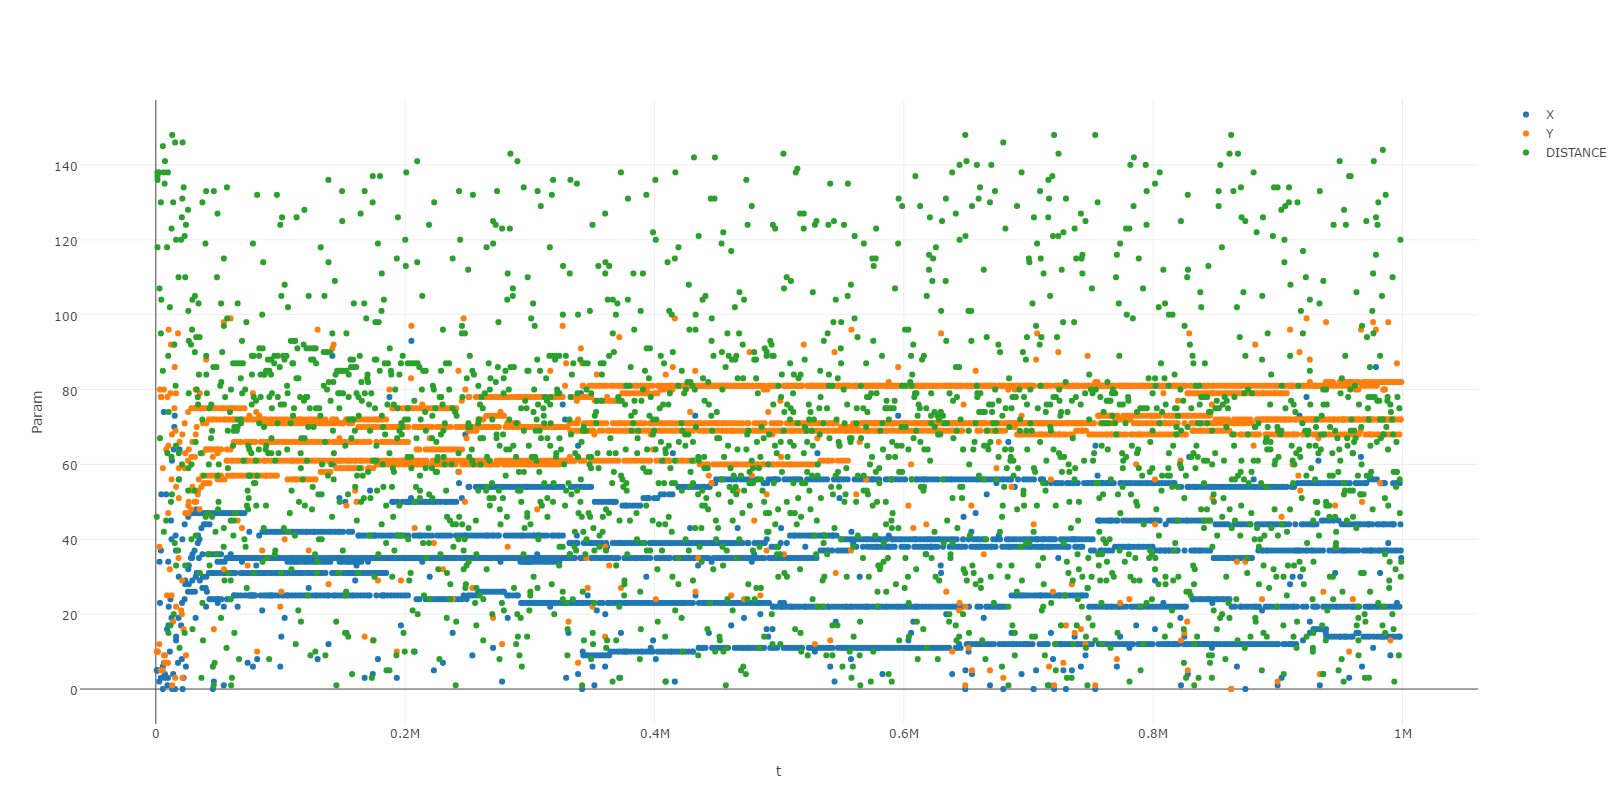
\includegraphics[width=0.8\textwidth]{analyse/SomeMutants/4pm/xy.png}
	\caption{\emph{X-Out-Of-Y}-Heuristik bei 4 Autos pro Minute und $20\%$ lernenden Fahrern}\label{fig:ap_pm_xy_4}
\end{figure}

\subsubsection*{Nur lernende Fahrer}
\begin{figure}[H]
	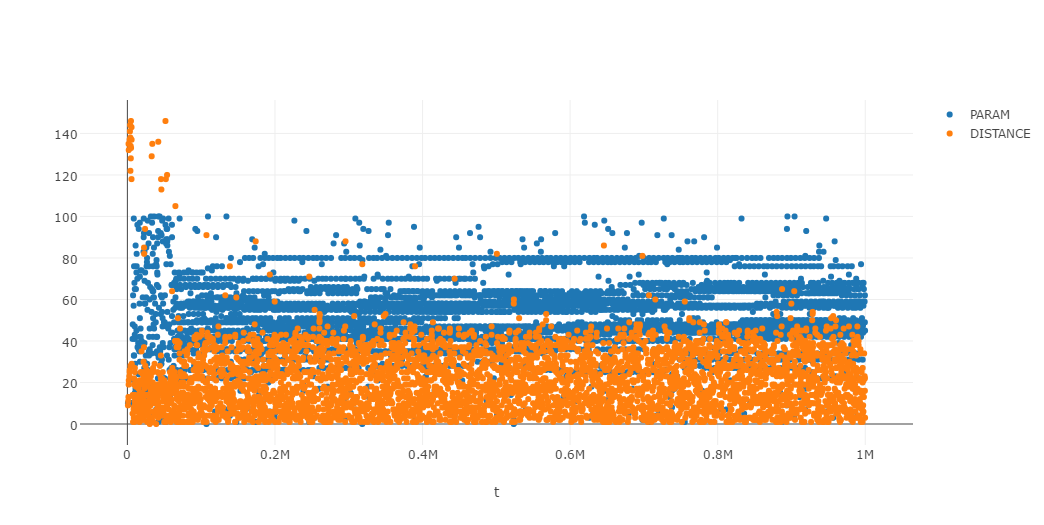
\includegraphics[width=0.8\textwidth]{analyse/JustHeuristik/1pm/block1just.png}
	\caption{\emph{Block-Count}-Heuristik bei 1 Auto pro Minute und nur lernende Fahrer}\label{fig:ap_jh_bs_1}
\end{figure}
\begin{figure}[H]
	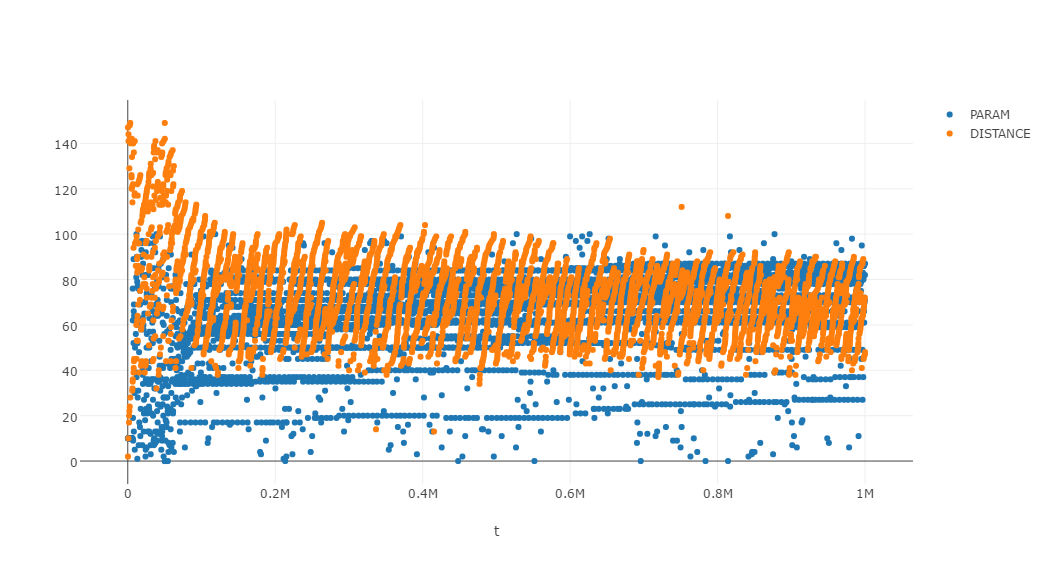
\includegraphics[width=0.8\textwidth]{analyse/JustHeuristik/1pm/car1just.png}
	\caption{\emph{Car-Count}-Heuristik bei 1 Auto pro Minute und nur lernende Fahrer}\label{fig:ap_jh_cc_1}
\end{figure}
\begin{figure}[H]
	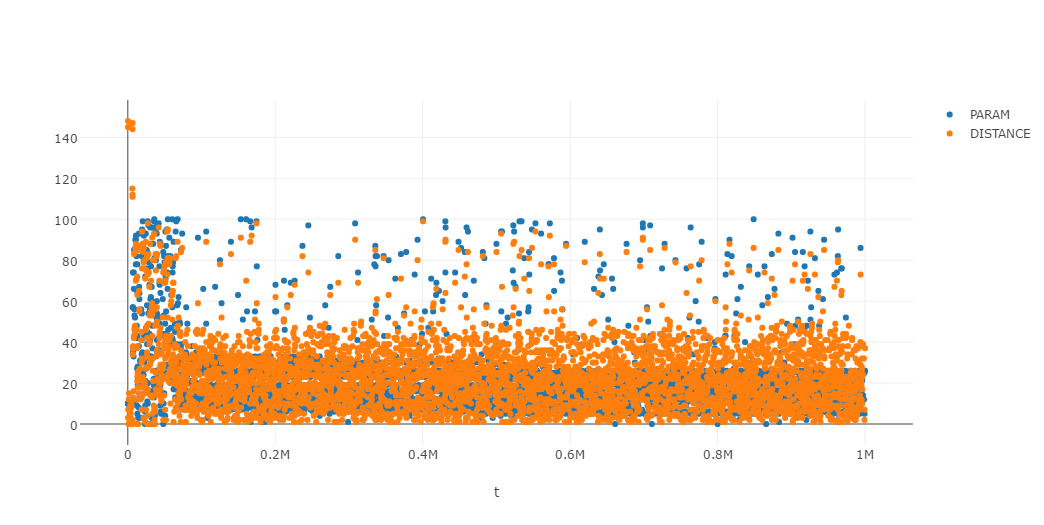
\includegraphics[width=0.8\textwidth]{analyse/JustHeuristik/1pm/fixed1just.png}
	\caption{\emph{Fixed-Distance}-Heuristik bei 1 Auto pro Minute und nur lernende Fahrer}\label{fig:ap_jh_fd_1}
\end{figure}
\begin{figure}[H]
	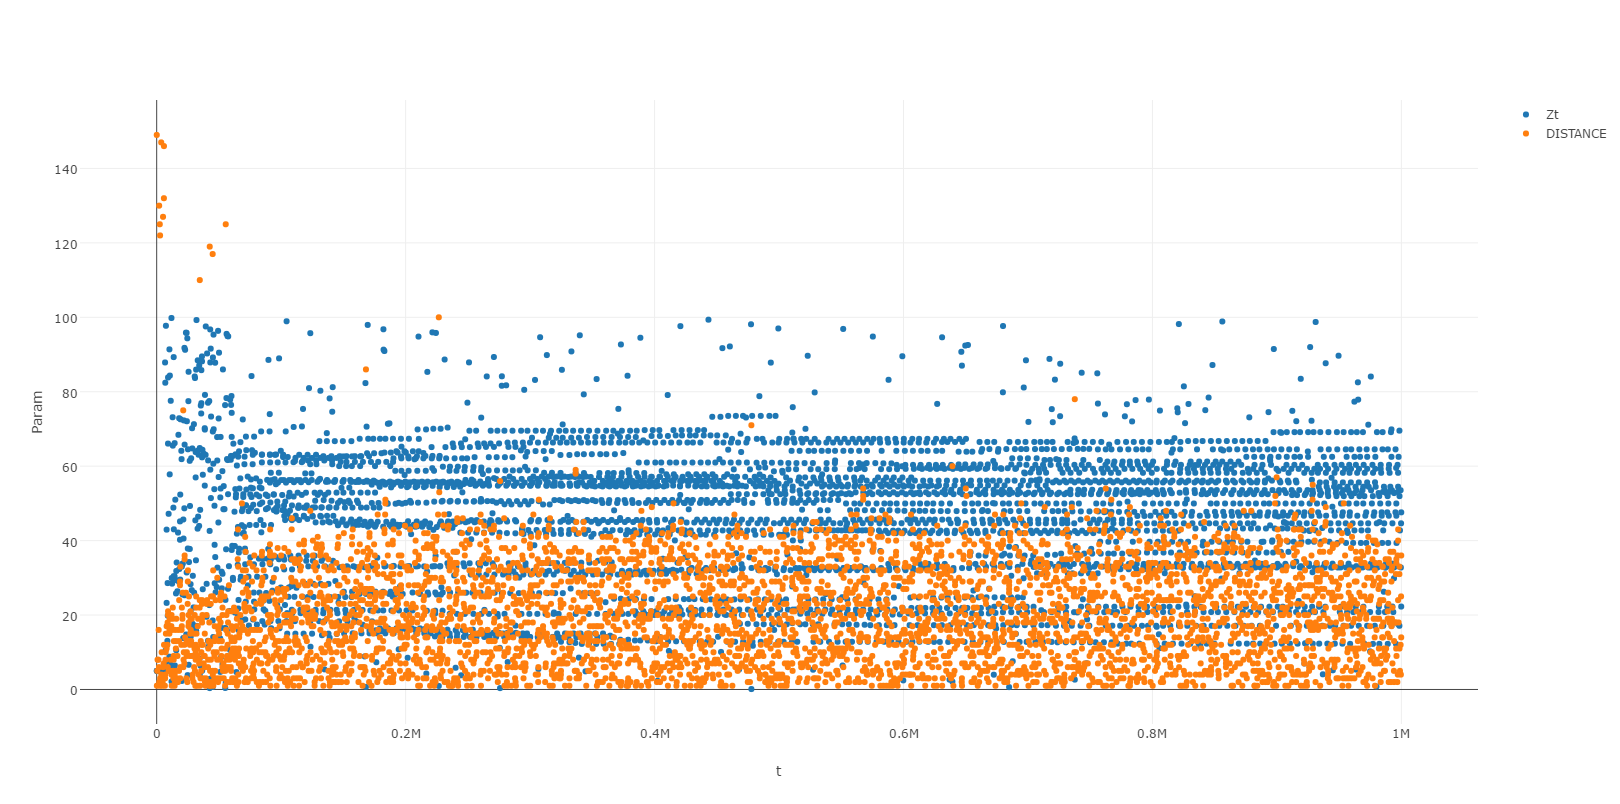
\includegraphics[width=0.8\textwidth]{analyse/JustHeuristik/1pm/linop.png}
	\caption{Schranke der \emph{Linear-Operator}-Heuristik bei 1 Auto pro Minute und nur lernende Fahrer}\label{fig:ap_jh_loz_1}
\end{figure}
\begin{figure}[H]
	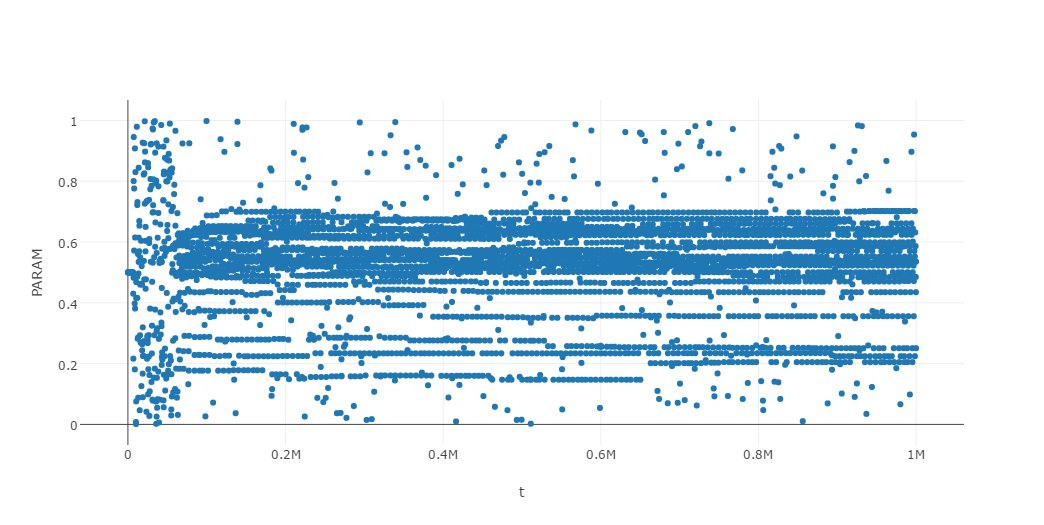
\includegraphics[width=0.8\textwidth]{analyse/JustHeuristik/1pm/linopa1just.png}
	\caption{Geschwindigkeit der \emph{Linear-Operator}-Heuristik bei 1 Auto pro Minute und nur lernende Fahrer}\label{fig:ap_jh_loa_1}
\end{figure}
\begin{figure}[H]
	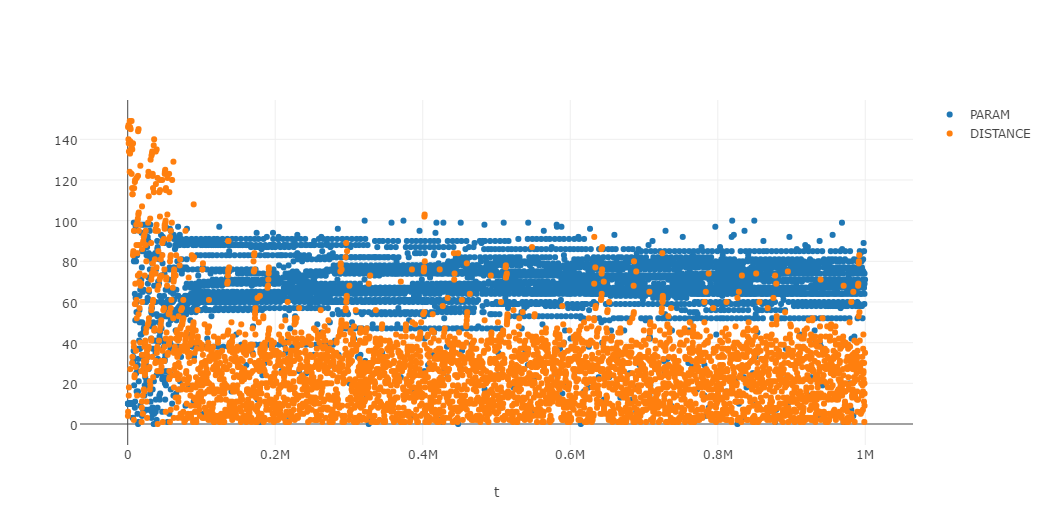
\includegraphics[width=0.8\textwidth]{analyse/JustHeuristik/1pm/space1just.png}
	\caption{\emph{Space-Count}-Heuristik bei 1 Auto pro Minute und nur lernende Fahrer}\label{fig:ap_jh_sc_1}
\end{figure}
\begin{figure}[H]
	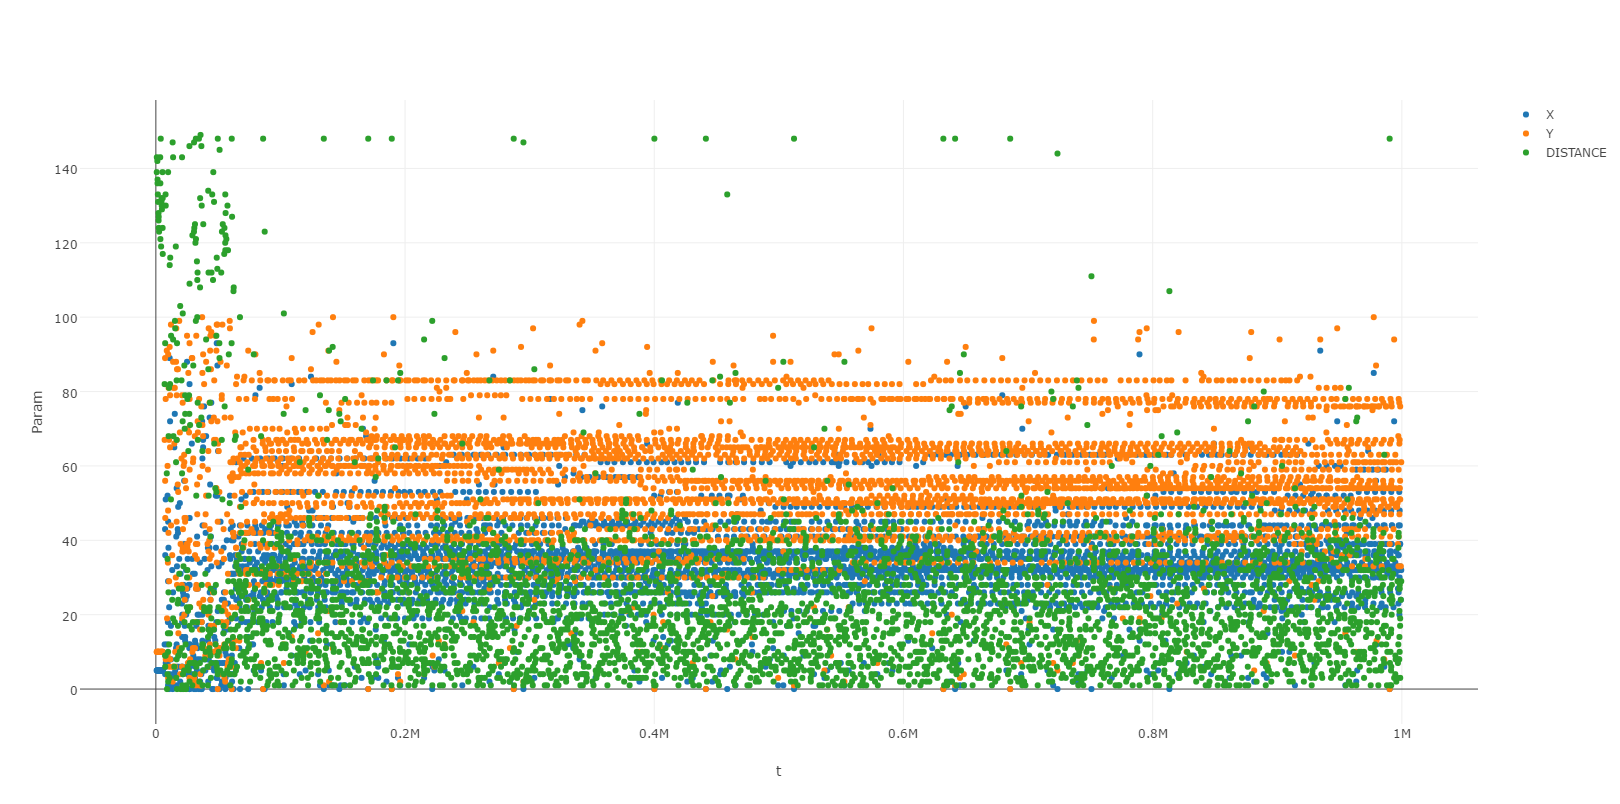
\includegraphics[width=0.8\textwidth]{analyse/JustHeuristik/1pm/xy.png}
	\caption{\emph{X-Out-Of-Y}-Heuristik bei 1 Auto pro Minute und nur lernende Fahrer}\label{fig:ap_jh_xy_1}
\end{figure}
\begin{figure}[H]
	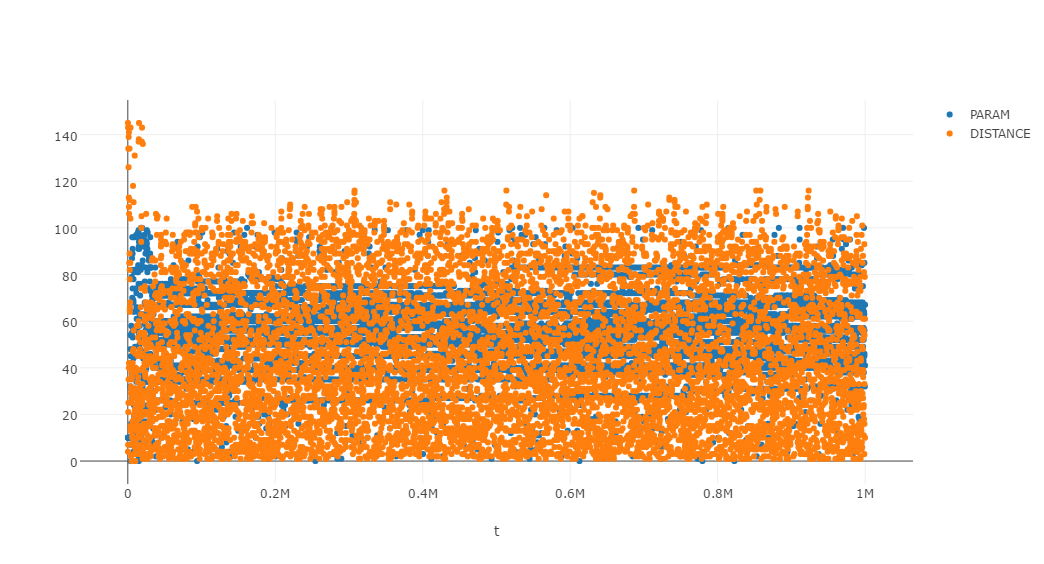
\includegraphics[width=0.8\textwidth]{analyse/JustHeuristik/2pm/block2just.png}
	\caption{\emph{Block-Count}-Heuristik bei 2 Autos pro Minute und nur lernende Fahrer}\label{fig:ap_jh_bs_2}
\end{figure}
\begin{figure}[H]
	\includegraphics[width=0.8\textwidth]{analyse/JustHeuristik/2pm/car2just.png}
	\caption{\emph{Car-Count}-Heuristik bei 2 Autos pro Minute und nur lernende Fahrer}\label{fig:ap_jh_cc_2}
\end{figure}
\begin{figure}[H]
	\includegraphics[width=0.8\textwidth]{analyse/JustHeuristik/2pm/fixed2just.png}
	\caption{\emph{Fixed-Distance}-Heuristik bei 2 Autos pro Minute und nur lernende Fahrer}\label{fig:ap_jh_fd_2}
\end{figure}
\begin{figure}[H]
	\includegraphics[width=0.8\textwidth]{analyse/JustHeuristik/2pm/linop.png}
	\caption{Schranke der \emph{Linear-Operator}-Heuristik bei 2 Autos pro Minute und nur lernende Fahrer}\label{fig:ap_jh_loz_2}
\end{figure}
\begin{figure}[H]
	\includegraphics[width=0.8\textwidth]{analyse/JustHeuristik/2pm/linopa2just.png}
	\caption{Geschwindigkeit der \emph{Linear-Operator}-Heuristik bei 2 Autos pro Minute und nur lernende Fahrer}\label{fig:ap_jh_loa_2}
\end{figure}
\begin{figure}[H]
	\includegraphics[width=0.8\textwidth]{analyse/JustHeuristik/2pm/space2just.png}
	\caption{\emph{Space-Count}-Heuristik bei 2 Autos pro Minute und nur lernende Fahrer}\label{fig:ap_jh_sc_2}
\end{figure}
\begin{figure}[H]
	\includegraphics[width=0.8\textwidth]{analyse/JustHeuristik/2pm/xy.png}
	\caption{\emph{X-Out-Of-Y}-Heuristik bei 2 Autos pro Minute und nur lernende Fahrer}\label{fig:ap_jh_xy_2}
\end{figure}
\begin{figure}[H]
	\includegraphics[width=0.8\textwidth]{analyse/JustHeuristik/4pm/block4just.png}
	\caption{\emph{Block-Count}-Heuristik bei 4 Autos pro Minute und nur lernende Fahrer}\label{fig:ap_jh_bs_4}
\end{figure}
\begin{figure}[H]
	\includegraphics[width=0.8\textwidth]{analyse/JustHeuristik/4pm/car4just.png}
	\caption{\emph{Car-Count}-Heuristik bei 4 Autos pro Minute und nur lernende Fahrer}\label{fig:ap_jh_cc_4}
\end{figure}
\begin{figure}[H]
	\includegraphics[width=0.8\textwidth]{analyse/JustHeuristik/4pm/fixed4just.png}
	\caption{\emph{Fixed-Distance}-Heuristik bei 4 Autos pro Minute und nur lernende Fahrer}\label{fig:ap_jh_fd_4}
\end{figure}
\begin{figure}[H]
	\includegraphics[width=0.8\textwidth]{analyse/JustHeuristik/4pm/linop.png}
	\caption{Schranke der \emph{Linear-Operator}-Heuristik bei 4 Autos pro Minute und nur lernende Fahrer}\label{fig:ap_jh_loz_4}
\end{figure}
\begin{figure}[H]
	\includegraphics[width=0.8\textwidth]{analyse/JustHeuristik/4pm/linopa4just.png}
	\caption{Geschwindigkeit der \emph{Linear-Operator}-Heuristik bei 4 Autos pro Minute und nur lernende Fahrer}\label{fig:ap_jh_loa_4}
\end{figure}
\begin{figure}[H]
	\includegraphics[width=0.8\textwidth]{analyse/JustHeuristik/4pm/space4just.png}
	\caption{\emph{Space-Count}-Heuristik bei 4 Autos pro Minute und nur lernende Fahrer}\label{fig:ap_jh_sc_4}
\end{figure}
\begin{figure}[H]
	\includegraphics[width=0.8\textwidth]{analyse/JustHeuristik/4pm/xy.png}
	\caption{\emph{X-Out-Of-Y}-Heuristik bei 4 Autos pro Minute und nur lernende Fahrer}\label{fig:ap_jh_xy_4}
\end{figure}